\documentclass{report}
\usepackage{hyperref}
\usepackage[ngerman]{babel}
\usepackage{amsmath}
\usepackage{amsfonts}
\usepackage{amsthm}
\usepackage{tcolorbox}
\usepackage[a4paper, total={7in, 9in}]{geometry}
\usepackage[font={scriptsize,it}]{caption}
\usepackage{scrextend}
\usepackage{graphicx}
\usepackage{caption}
\usepackage{subcaption}
\usepackage[utf8]{inputenc}
\usepackage[T1]{fontenc}
\DeclareUnicodeCharacter{2212}{-}
\usepackage{verbatim}
\usepackage{tikz}

\tikzset{
  treenode/.style = {shape=rectangle, rounded corners,
                     draw, align=center,
                     top color=white, bottom color=blue!20},
  root/.style     = {treenode, font=\Large, bottom color=red!30},
  env/.style      = {treenode, font=\ttfamily\normalsize},
  dummy/.style    = {circle,draw}
}

\tikzstyle{level 1}=[level distance=3.5cm, sibling distance=3.5cm]
\tikzstyle{level 2}=[level distance=3.5cm, sibling distance=2cm]

% floating figure for column
\newenvironment{Figure}
	{\par\medskip\noindent\minipage{\linewidth}}
	{\endminipage\par\medskip}

\theoremstyle{definition}
\newtheorem{definition}{Definition}

\theoremstyle{example}
\newtheorem*{example}{Example}

\begin{document}

\begin{titlepage}
   \vspace*{\stretch{1.0}}
   \begin{center}
      \Large\textbf{Natural User Interfaces - HS20}\\
      \large\textit{Pascal Brunner - brunnpa7}
   \end{center}
   \vspace*{\stretch{2.0}}
\end{titlepage}

% Beispiel Bild
%\begin{Figure}
%   \centering
%    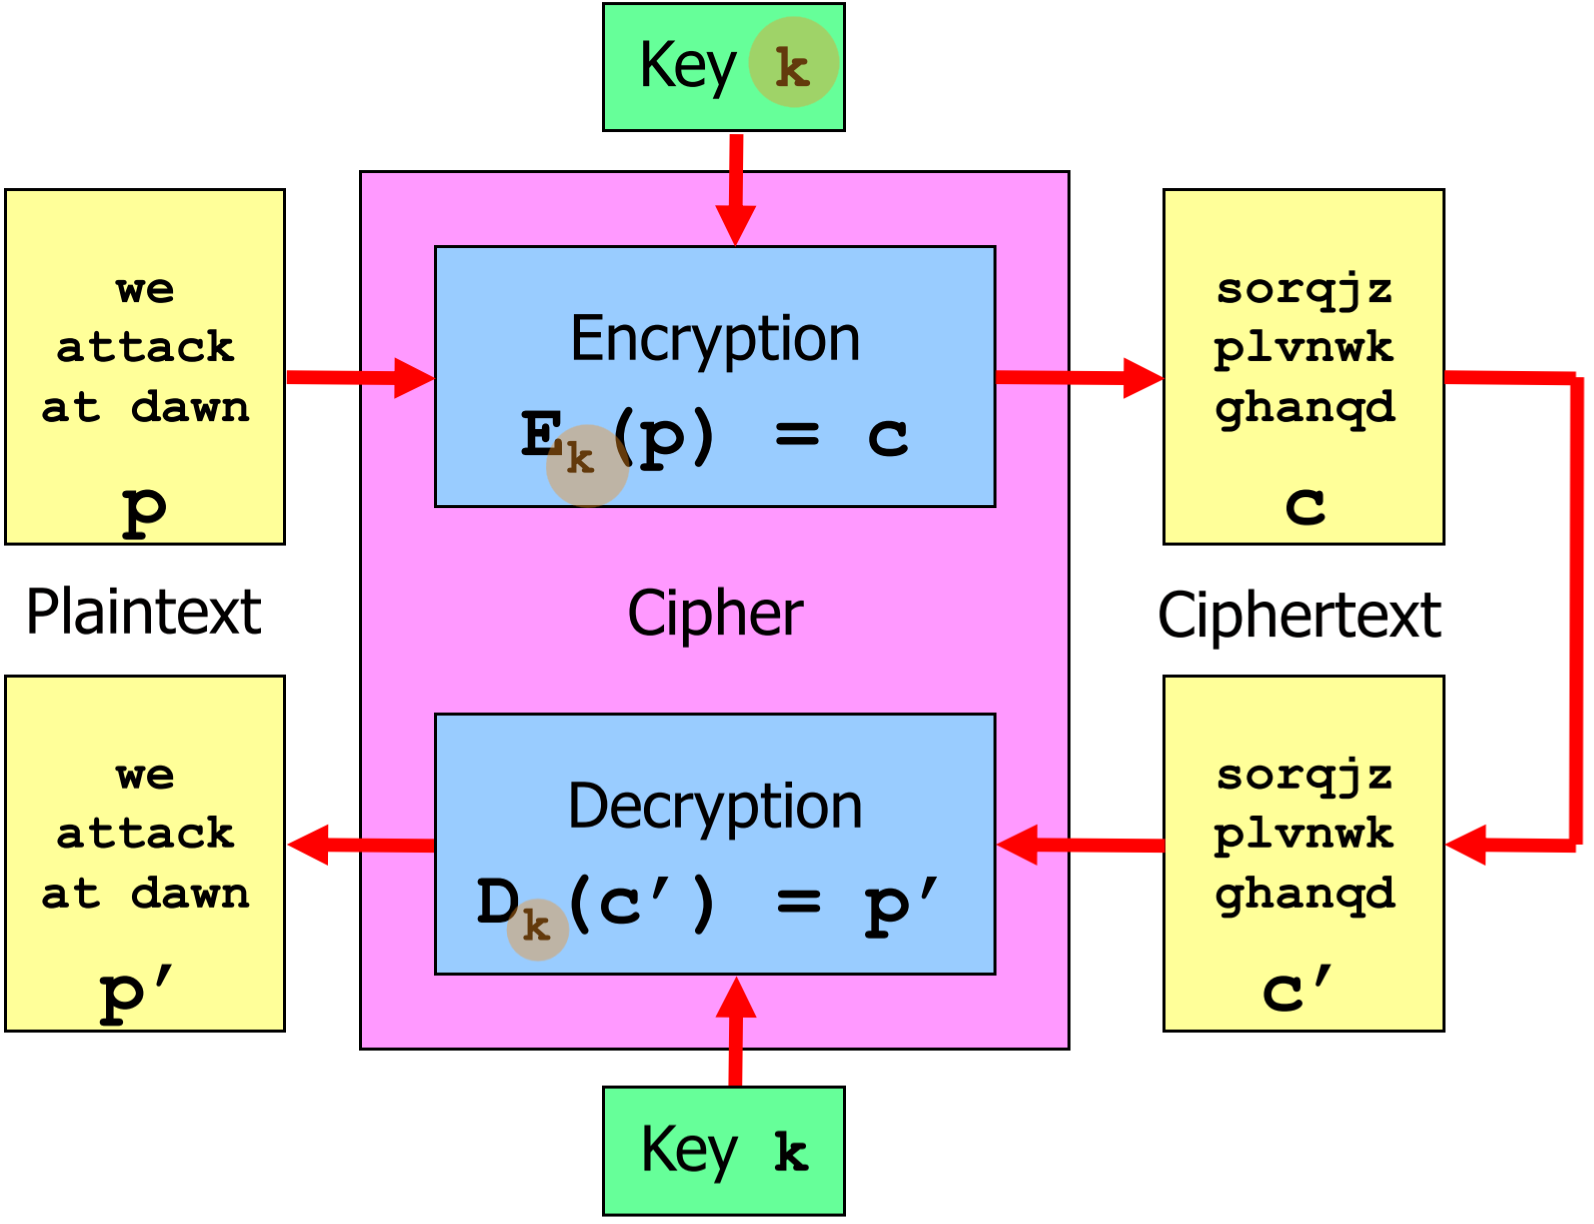
\includegraphics[width=150px]{img/BasicTerminologySecKeyCrypto.png}
%        \captionof{figure}{Basic Terminology basierend auf Secret Key Cryptography}
%        \label{fig:Basic Terminology}
%    \end{Figure}

\tableofcontents

\newpage

\chapter{From GUIs to NUIs}

\section*{Graphic User Interface (GUI)}
\subsection{Text-based UIs}
\begin{itemize}
   \item Beispielsweise Terminal
   \item Designed, damit man nicht zu schnell tippen kann
\end{itemize}

\subsection{Klassisches GUI}
\begin{itemize}
   \item Input: Keyboard, Mouse, Pen
   \item Output: Displays
\end{itemize}

\subsubsection{WIMP-Paradigma}
Basiert auf dem WIMP-Paradigma
\begin{itemize}
   \item Windows $\rightarrow$ modal (alles andere blockiert - bspw. Speicher-Fenster) / nicht-modal (kann anderweitig weiterarbeiten - Suchfenster im Word)
   \item Icons $\rightarrow$ für Dokumente, Programme
   \item Menus $\rightarrow$ für Befehle und Auswahl
   \item Pointer $\rightarrow$ Pointing, Selecting, Activating, Drawing, dragging
\end{itemize}

\subsubsection{Metaphern}
\begin{itemize}
   \item Desktop
   \item Files und Folders
   \item Recycle bin
\end{itemize}

\subsubsection{Widget}
\begin{itemize}
   \item Buttons
   \item Sliders
   \item etc
\end{itemize}

\subsection{3 Prinzipien der direkten Manipulation}
\begin{itemize}
   \item \textbf{Continuous} representations of objects and actions of interest with meaningful visual methaphors
   \item \textbf{Physical Actions} (e.g. dragging) instead of complex syntac
   \item \textbf{Rapid, incremental, reversible (undo) actions} whose effects on the objects of interest are immediately visible (WYSIWYG)
\end{itemize}

\textit{Beispiel Dokument unbenennen}
\begin{itemize}
   \item \textbf{Continuous representations} $\rightarrow$ Icon bzw. Dokument bleibt ersichtlich
   \item \textbf{Physical Actions} $\rightarrow$ neuer Namen kann einfach eingetragen werden
   \item \textbf{Rapid, incremental, reversible (undo) actions} $\rightarrow$ Falls man doch nicht unbennen will, kann man einfach die Aktion stoppen
\end{itemize}

\subsection{Vor- / Nachteile GUIs}
\textbf{Vorteile}
\begin{itemize}
   \item Visual representations of task concepts
   \item allows easy learning
   \item allows easy retention
   \item allows errors to be avoided
   \item encourages exploration
   \item affords high subjective satisfaction
   \item allows immediate feedback
\end{itemize}

\textbf{Nachteile}

\begin{itemize}
   \item Direct Manipulation is indirected by mouse, trackpad, etc $\rightarrow$ large translational distance
   \item High computational demand
   \item accdessibility is a challenge
   \item automation of tasks more challenging
\end{itemize}

\section*{Natural User Interfaces (NUI)}
Wieso braucht es mehr als das WIMP-Prinzip?\\
$\rightarrow$ WIMP ist nicht geeignet für kleine, mobile oder 'unsichtbare' Computers

\subsection{Charakteristik}
\begin{itemize}
   \item Die Bedingung soll so natürlich wie möglich sein
   \item Gerade für den Touchscreen wichtig
   \item allow multimodal interaction $\rightarrow$ sehr natürlich für die Anwender, da Menschen immer Multimodal agieren (Sprechen, Gestik, Mimik alles gleichzeitig)
   \item are context aware $\rightarrow$ From context of task to context of usage $\Rightarrow$ Can significantly improve mobile applications and user assistance
\end{itemize}

\begin{Figure}
   \centering
    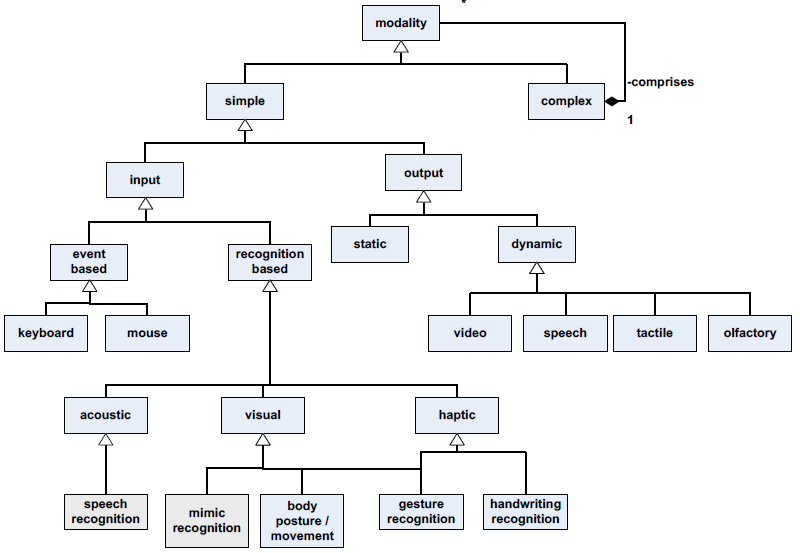
\includegraphics[width=150px]{img/OverviewModalities.png}
        \captionof{figure}{Übersicht über die verschiedenen Arten der Modalitäten}
        \label{fig:Overview Modalities}
\end{Figure}

   \subsection{Main issues of the new modalities}
   tbd

   \subsection{Ziele}
\begin{itemize}
   \item reduces translational distance (more direct Manipulation)
   \item fits basic skills of users
   \item feel natural from the beginning
   \item all in all: improve usability
\end{itemize}

\section*{Usability}
\begin{itemize}
   \item Usability $\rightarrow$ Wie einfach kann ich die Anwendung verwenden (Deutsch: Gebrauchstauglichkeit)
   \item User Experience (UX) $\rightarrow$ Look and feel der Anwendung 
   \item Customer Experience $\rightarrow$ Usability + Desirability + Brand Experience
\end{itemize}
\begin{Figure}
   \centering
    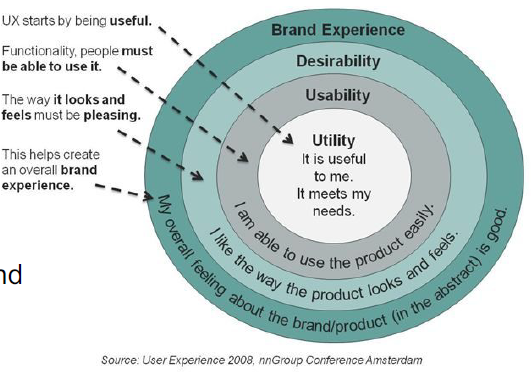
\includegraphics[width=150px]{img/Usability.png}
        \captionof{figure}{Usability}
        \label{fig:Usability}
\end{Figure}

\textbf{Definition nach DIN ISO 9241}: The effectiveness, efficiency and satisfaction with which specified users achieve specified goals in particular environments

\subsection{Die drei wichtigsten Anforderungen rund um die Usability (auch Usability Engineering genannt)}
\begin{itemize}
   \item zu Deutsch: Ergonomie
   \item Effektiv $\rightarrow$ die Aufgabe kann komplett abgeschlossen werden
   \item effizient $\rightarrow$ mit möglichst wenig Aufwand
   \item Zufriedenheit $\rightarrow$ Es soll Spass machen die Aufgabe zu erfüllen
\end{itemize}

\subsection{Die sieben wichtigsten Charakteristiken}
\begin{itemize}
   \item Suitability for the task (Aufgabenangemessenheit)
   \item Suitability for learning (Lernförderlichkeit)
   \item Suitability for indivualisation (Individualisierbarkeit) $\rightarrow$ Experte möchte schneller sein als Anfänger
   \item Conformity with user expectation (Erwartungskonformität)
   \item self descriptiveness (Selbstbeschreibungsfähigkeit) $\rightarrow$ UI ist selbst erklärend
   \item Controllability (Steuerbarkeit)
   \item Error tolerance (Fehlertoleranz)
\end{itemize}

\subsubsection{self Descriptiveness}
\begin{itemize}
   \item genügend Informationen zur Verfügung stellen
   \item Consider user's knowledge
   \item Terminologie an die Domäne angepasst
   \item Bestätigung anfordern vor kritischen Aktionen
   \item Erschwinglichkeit
   \item Mapping
\end{itemize}

\subsubsection{suitability for the task}
\begin{itemize}
   \item Möglichst wenig Schritte für die jeweilige Aufgabe
   \item Nur die notwendigen Informationen für den jeweiligen Prozessschritt angeben
   \item Kontext-abhängige Hilfe
   \item möglichst wenig User-input wie möglich
   \subitem same input only once
   \subitem standardwerte
   \subitem vordefinierte Liste für Eingabe (bspw. Länder)
\end{itemize}

\subsubsection{Controllability}
\begin{itemize}
   \item Dialog sollte durch den User bestimmt werden
   \item Alle Dialogschritte sollten eine undone-Funktion beinhalten
   \item Möglichkeit anbieten um Aktionen zu canceln
\end{itemize}

\subsubsection{Conformity to expectations}
\begin{itemize}
   \item Betreffend folgenden Punkten
   \subitem Designe
   \subitem Interaktion
   \subitem Struktur
   \subitem Komplexität
   \subitem Funktion
   \item Terminologie, welche für den USer bekannt sind
   \item Verhalten 
   \item Präsentation der Informationen 
   \subitem bspw. Reihenfolge der Benutzereingaben (Name, Adresse etc.) 
\end{itemize}

\subsubsection{Error Tolerance}
\begin{itemize}
   \item Fehler vermeiden (Validätskontrolle)
   \item Gewisse Aktionen in den bestimmten Situation ein oder ausblenden
   \item Hilfestellung für den User liefern
   \item Einfache Möglichkeit den Fehler zu korrigieren
   \item Auf keinen Fall sollte was verloren gehen, was der User bereits gemacht hat
\end{itemize}

\subsubsection{Suitability of Individualisation}
\begin{itemize}
   \item Sollte für alle User anwendbar sein
   \subitem Level des Users
   \subitem Allfällige Einschränkungen
   \subitem Sprachen 
\end{itemize}

\subsubsection{Learnability}
\begin{itemize}
   \item Das System sollte dem User Informationen zu den darunterliegenden Konzepte und Regeln liefern
   \subitem Tool-Tips
   \subitem Tutorials
   \item Die Basis Funktionalität sollte bedienbar sein, ohne ein Tutorial machen zu müssen
\end{itemize}

\section*{User Centered Design (UCD)}
Eine Möglichkeit wie man das Design angehen kann

\subsection{Begrifflichkeiten}
\begin{itemize}
   \item User Experience Design $\rightarrow$ Alle Aspekte der Interaktion
   \item User-centered Design $\rightarrow$ 
   \item User interface Design $\rightarrow$ interface zwischen User und System
   \item 
\end{itemize}

\subsection{UCD Prozess}
\begin{Figure}
   \centering
    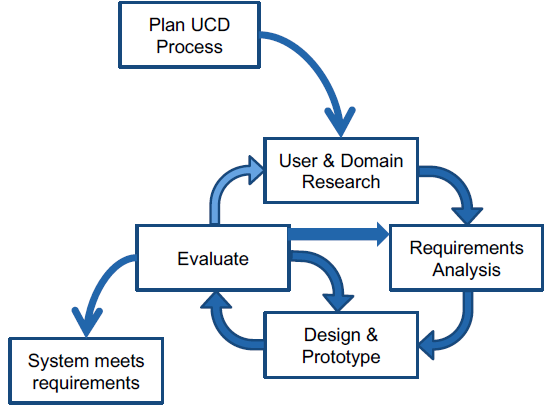
\includegraphics[width=150px]{img/UCD Process.png}
        \captionof{figure}{Prozessablauf}
        \label{fig:UCD Process}
\end{Figure}
\begin{itemize}
   \item User und Domain Research
   \subitem Zielgruppe und Domäne definieren
   \subitem Aufnahme möglicher Anforderungen
   \item Requirement Analysis
   \subitem Aufgaben, Kontext, ...
   \item Design und Prototype
   \item Evalutation
\end{itemize}

\subsubsection{User and Domain Research}
Wichtigste Phase: Man muss den User und den Kontext verstehen!

\begin{itemize}
   \item User verstehen
   \item Kontext verstehen
   \item klares Verständnis über das Business
\end{itemize}

\textbf{User verstehen}\\
\begin{itemize}
   \item Wer sind die Users?
   \item Was ist ihre Arbeit, Aufgaben und Ziele?
   \item Was ist der Kontext ihrer arbeit?
   \item Was brauchen Sie um die Ziele zu erreichen?
   \item Wie ist die Domänensprache?
   \item Normen (Organisatorisch etc.)
   \item Pain Points im Workflow
\end{itemize}

\textbf{Kontext verstehen}\\
\begin{itemize}
   \item Wo wird die App verwendet?
   \item Wann wird die App verwendet?
   \item Wieso wird die App verwendet?
\end{itemize}

\textbf{Personas}\\
Ist eine fiktionale Person, welche eine Gruppe repräsentiert. Dies ist sehr wichtig und gilt als Grundlage für die nächsten Diskussionen.\\

\textbf{Usage Scenarios}\\
Beschreibt den \textbf{aktuellen} Ablauf, beziehungsweise an allfälliger Use-Case. Dabei gibt es immer die gleichen Aspekte
\begin{itemize}
   \item title
   \item Kontext
   \item Trigger
   \item Ziel
   \item Aktion und Interaktion
\end{itemize}

\textbf{Artefakten}
\begin{itemize}
   \item Personas
   \item Usage Scenarios
   \item Mental Model
   \item Domain Model
   \item Stackholder Map $\rightarrow$ Wer interagiert, wie stark mit der App
   \item Business Process Model
   \item Service Blueprint
\end{itemize}

\subsubsection{Requirement Analysis}
\begin{itemize}
   \item Beschreibt was man in der Zukunft möchte
   \item Kann nicht einfach gesammelt werden
   \item Keine Features
   \item Keine Spezifikationen
\end{itemize}

\textbf{Context Scenario}\\
\begin{itemize}
   \item Beschreibt Zukunft 
   \item Beschreibung ist optimistisch
   \item textliche und in Form einer Geschichte
   \item aus User-perspektive aus Persona-Sicht
   \item Braucht folgende Punkte
   \subitem Motivatino, Trigger
   \subitem Persona
   \subitem Kontext
   \subitem Ablenkungen
   \subitem Ziel
\end{itemize}

\begin{enumerate}
   \item Szenarios identifizieren für jede Persona
   \item Erarbeitung der einzelnen Stories
   \item Anforderungen ableiten
\end{enumerate}

\subsubsection{UI Design and Prototype}
Design einer möglichen Lösung basierend auf den Anforderungen, welche die Ziele effektiv, effizient und zufriedenstellend abdecken.

\subsubsection{Evaluate}
Testen und evaluieren des UI-Prototypes, mit echten Anwendern und / oder Usability Experten

\chapter{UCD: Conceptual Design and Prototype}
Das Hauptziel ist, dass man ein passendes Design-Konzept hat.\\
\begin{itemize}
   \item Einigung auf die Design-Prinzipien
   \subitem Charakteristik beschreiben des Produkts mit ein paar Statements
   \subitem kurz und bündig 
   \subitem App Definition Statement $\rightarrow$ bei einer Android-App ist das beispielsweise einen Satz (Was? für wen? welchen (Mehr-)wert? Kontext?)
   \item Sources
   \item Wie: Workshop mit dem Design-Team und Stakeholder
\end{itemize}

\section{Ablauf eines Conceptual Design}
\begin{enumerate}
   \item Interaktion Styles, Posture nud Interaktion Pattern auswählen
\end{enumerate}

\subsection{Interatcion Styles}
Können Prozess- oder Produkt-orientiert sein.\\
\textbf{Proezss-orientiert}:
\begin{itemize}
   \item Instructing
   \item Form filling $\rightarrow$ System fragt Daten ab
   \subitem Für effizienten Daten-input via Text-Feld und Auswahl (bspw. Webformulare oder Login)
   \item Conversing $\rightarrow$ Konversationen führen mit dem System
   \subitem User fragt, System Antwortet (text oder speech) (bspw. Chatbot, Suchmaschinen, Roboter)
   \item Manipulating / Navigating
   \subitem Virtuelle Umgebung von Objekten (bspw. Direkte Manipulation auf dem GUI $\rightarrow$ Desktop)
   \subitem Man kann navigieren, auswählen, öffnen, zoomen etc.
   \item Exploring / Browsing 
   \subitem Suchen und Finden von Informationen (Bspw. Webseiten)
\end{itemize}

\textbf{Produkt-orientiert}
\begin{itemize}
   \item Direkte Interaktion mit einem Objekt
   \subitem Analogie zu 'echten Objekten' (Bspw. Excel, Zahlungsapplikationen, Kompass-App)
\end{itemize}

\subsection{Application Posture}
\begin{itemize}
   \item Sovereign $\rightarrow$ Applikation dominiert den screen (bspw. PowerPoint, Excel)
   \item Transient $\rightarrow$ Für eine spezifische Aufgabe (sind die meisten Apps, bspw. Rechner auf dem Handy)
   \item Daemonic $\rightarrow$ Arbeitet die meiste Zeit im Hintergrund (bspw. Firewall, Anti-Virus-System)
   \item Auxiliary $\rightarrow$ Bleibt aktiv über eine lange Zeit (bspw. Toolbar, media Player)
\end{itemize}

\subsection{Interaction Pattern}
Sind Lösungen für verschiedene Interaktionsprobleme\\
Diese Pattern werden häufig miteinander kombiniert (bspw. MS Outlook organizer + tab)

\subsubsection{Command-Line}
$\Rightarrow$ Textliche Konversation\\
Vorteil: 
\begin{itemize}
   \item Effizient und flexibel
   \item Sehr mächtig
   \item Sehr gut für Experten
\end{itemize}
Nachteile:
\begin{itemize}
   \item Nicht einfach zu lernen
   \item schlecht für Anfänger
\end{itemize}

\subsubsection{Forms}
Textliche Konversation, das System fragt explizit die Informationen ab\\
Vorteil: 
\begin{itemize}
   \item Einfach zu lernen
   \item Effizient für die Dateneingabe (mit Tastatur)
   \item Sehr flexibel
\end{itemize}
Nachteile:
\begin{itemize}
   \item Weniger effizient für Touch-Interaktionen
   \item Fehleranfällig (Typos etc.)
\end{itemize}

\subsubsection{Organizer / workspace}
Zwei panes (1x Organizer, 1x Workspace) bspw. PowerPoint, Outlook etc.

\subsubsection{Parallel workspaces}
\begin{itemize}
   \item erlaubt schnelles Wechseln der Workspaces 
   \item Sehr sinnvoll, wenn man mehrere Aufgaben bearbeiten muss
   \item Meistens mit Tabs implementiert
   \item Bspw. Ribbons in Office
\end{itemize}

 \subsubsection{Wizard (tunnel)}
 Der User führt genau eine spezifische Abfolge von Aktionen durch, wobei der User nur vor und zurück kann. 
 Wird vor allem für kritische Aufgaben verwendet (bspw. Software-Installation)

 \subsubsection{Multi Document Interface (MDI)}
 ein Hauptwindow und erlaubt mehrere child-windows\\
 $\rightarrow$ wird sehr häufig in desktop Applikationen verwendet (bspw. mehrere Word-Fenster offen)

 \subsubsection{1st person environment}
 Man sieht die Umgebung wie aus einer eigenen perspektive, wie man dort stehen würde
 \begin{itemize}
    \item video games
    \item google street 
    \item Schach
    \item Immersive Environment
 \end{itemize}

 \subsubsection{3rd person Environment}
 Der Anwender sieht von aussen auf die Applikation drauf. Wird häufig für Schulanwendungen verwendet.

 \subsubsection{Hub-And-Spoke}
 \begin{itemize}
    \item Nabe und Speichern
    \item hierarchisches Menü
    \subitem bspw. Mobile-Geräte Gruppieren von Apps, durch das klicken in den App-Ordner, kann man anschliessend die gewünschte App auswählen 
    \item Sehr häufig bei mobilen Geräte verwendet
 \end{itemize}

 \subsection{Metaphern}
 Beispielsweise das Konzept des Warenkorbs in Online-Shops oder der Papierkorb.\\
 dadurch hat man relativ schnell das Interaktionskonzept definiert, jedoch muss man aufpassen, dass es durch die ganz Applikation konsistent ist\\
 Sehr häufig werden dann mehrere Konzepte miteinander verbunden, da es nicht immer 1:1 übernommen wird - bspw. Fenster (Frische Luft kann man nicht reinlassen im virtuellen Fenster, jedoch kann man es öffnen und schliessen)

 Man muss jedoch aufpassen, dass man nicht kulturulle Regeln nicht verletzt. (gibt noch weitere Sachen) $\Rightarrow$ kann zu Problemen führen

\subsection{Daten-Objekte identifizieren}
Ein Daten-Objekt hat jeweils folgende Typen
\begin{itemize}
   \item Object-Type (bspw. TimeSlots)
   \item Definition (bspw. Uninterrupted period of time)
   \item Relationsship (bspw. StartDate, EndDate, StartTime, EndTime)
   \item States (bspw. Proposed)
   \item Actions (bspw. CRUD, addVote, removeVote)
   \item Attributes (bspw. NumVotes, Comment)
\end{itemize}

...

\subsection{Function Blocks and Screens}
\begin{enumerate}
   \item Als erstes soll durch die wichtigsten Kontext-Szenarien durchgegangen werden (Funktionen und Daten identifizieren welche gebraucht werden)
   \item ...
\end{enumerate}

\subsubsection{Storyboarding Screens and Navigation}
\begin{itemize}
   \item mit dem Hauptanwendungsfall und der primären Persona beginnen
   \item Entscheidung welches Interaktionspattern
   \item Nur thumbnails (empty or named rectangles)
   \item Szenario Flow suggests position (Top-down, left-right)
   \item Object nature suggests size and shape
   \item Prozedere mit einem anderen Kontext-Szenario und der primären Persona durchgehen
   \item Probiere Screens zu konsolidieren
   \item Entwicklung eines groben Storyboards für alle key path scenarios
\end{itemize}

\subsection{Touch Interaction Patterns}

\subsubsection{Gestures}
\textbf{Tab (touch)}
\begin{itemize}
   \item Touch with one finger
   \item simplest manual touch Gestures
   \item activate-on-press 
   \item activate-on-release (Better to touch) 
   \item press-and-hold
\end{itemize}

\textbf{Tap to select}: object, menu item, list item\\
\textbf{tap to activate}: button, menu, link, app\\

\textbf{Double-Tap}
\begin{itemize}
   \item Onto an object / into an area 
   \item to zoom in / out 
   \item To select 
   \item to activate / open
\end{itemize}

\textbf{Long-Press}
\begin{itemize}
   \item Onto an object / into an area 
   \item to show context menu 
\end{itemize}

\textbf{Drag (Pan)}
\begin{itemize}
   \item Drage one finger over the screen (move object, drag-and-drop etc)
   \item combined with tap, double-tap, long-press
   \item Wichtig! Sofortiges Feedback
\end{itemize}

\textbf{Slide}
\begin{itemize}
   \item Continuous movement, similar to pan
   \item Movement restricted to horizontal/vertical
   \item to scroll screen, list of items slowly
   \item wichtig sofortiges visuelles Feedback
\end{itemize}

\textbf{Slide and Hold}: for Continuous scrooling (wichtig sofortiges Feedback)\\

\textbf{Fling (Swipe)}
\begin{itemize}
   \item to browse a list
   \item to scroll a screen
   \item exhibits a momentum
   \item movement often restricted
\end{itemize}

\textbf{Flick}
\begin{itemize}
   \item To brows a list quickly
   \item To scroll a page quickly
   \item ...
\end{itemize}

\textbf{Pinch}
\begin{itemize}
   \item Two finger tips move closer to eachother on an object / screen
   \item to shrink object / view (zoom out)
\end{itemize}

\textbf{Spread}
\begin{itemize}
   \item two finger tips move away from eachother on an object / screen
   \item to enlarge object / view (zoom in)
\end{itemize}

\subsubsection{Navigation}
\begin{itemize}
   \item Springboard (Hub and Spoke)
   \item Cards 
   \item List Menu 
   \item Tab Menu 
   \item Gallery
   \item Dashboard
   \item Methaphor / Skeumorphism
\end{itemize}

\section{Prototype}

\begin{itemize}
   \item Low fidelity
   \subitem Sketches
   \subitem Storyboards
   \subitem Paper Prototypes
   \subitem wireframes (klickbar) 
   \item High fidelity
   \subitem SW Prototype
   \subitem Video Prototype
\end{itemize}

\subsection{Low Fidelity}
\begin{enumerate}
   \item Als erstes mit Stift und Papier
   \item Überführung in einem prototyping tool (Balsamiq, Marvelapp)
\end{enumerate}

\subsection{Evaluieren}
Durch den Prototype evaluiert man sein Design, idealerweise direkt mit echten Usern. Die User erhalten eine Aufgabe (bspw. mache einen Termin ab mit der App)\\
How to do:
\begin{itemize}
   \item Moderator erklärt
   \subitem die Aufgabe und das Ziel 
   \subitem Wie der Prototype funktioniert
   \item Tester
   \subitem Führt die Aufgabe durch
   \subitem Denkt laut (Sehr wichtig)
   \item Papier prototype 
   \subitem zweite Person gibt dem Tester die Screens welcher er faktisch klicken würde
\end{itemize}
$\rightarrow$ ist ein iterativer Prozess bis man das optimal UI-Design Concept hat

\chapter{Usability Guidlines}

\section{8 goldige Regeln von Ben Shneiderman}

\begin{enumerate}
   \item Streben nach Konsistenz
   \subitem gleiche Aktionen, sollen gleich bedient werden
   \subitem konsistente Befehle 
   \item Anbieten von Shortcuts
   \item informatives Feedback liefern
   \item Dialoge sollen so gestaltet werden, dass sie abgeschlossen werden Können
   \subitem Sequenzen nach ihren Aktionen gruppieren bspw. Anfang, Mitte und Ende
   \subitem Es ist mental weniger anstrengend für die Bedienenden
   \item Fehler verhindern und einfaches Fehlerhandling
   \subitem als erstes sollen Fehler grundsätzlich verhindert werden
   \subitem als zweites sollen Fehler frühzeitig erkannt werden
   \subitem tbd
   \item Anbieten von undo-Funktion
   \subitem NUIs: Ist schwierig für Gesten
   \item Unterstützung des internen locus
   \subitem Man möchte eine Aufgabe erledigen und nicht sich mit dem Computer auseinanderzusetzen
   \subitem Man möchte nicht das Gefühl des Beifahrers haben
   \item  Reduzieren sie die Last des Kurzzeitgedächnises
\end{enumerate}

\section{10 Heuristics of Jacob Nielsen}
Jacob Nielsen ist einer der Usability-Gurus

\begin{enumerate}
   \item Visibility of system status
   \item Übereinstimmung von Systemen und der realen Welt
   \subitem Sollte sich an dem Domänenmodell bezgl. Begrifflichkeiten und Umgebung anlehnen 
   \item Benutzerkontrolle und Freiheit
   \subitem Anbieten eines \textit{emergency exit} um aus einem ungewollten Zustand zu gelangen
   \subitem support undo und redo
   \subitem NUIs: schwierig für Gesten 
   \item Konsistenz und Standard
   \subitem wörter, sätze und aktionen konsistent verwenden 
   \item Fehler vermeiden
   \item Erkennung statt Erinnerung
   \subitem Affordances
   \item Flexibilität und Effizient der Benutzung (Analog Shneiderman: Shortcuts)
   \subitem Accelerators 
   \item Aesthetic und minimales Design
   \subitem irrelevante Informationen weglassen
   \item Usern helfen Fehler zu erkennen, zu diagnostizieren und erholen von Fehlern
   \item Helfen und Dokumentation 
\end{enumerate}

\section{Touch interfaces}
Es gibt unterschiedliche Art und Weise wie man das Smartphone bedient.
\begin{Figure}
   \centering
    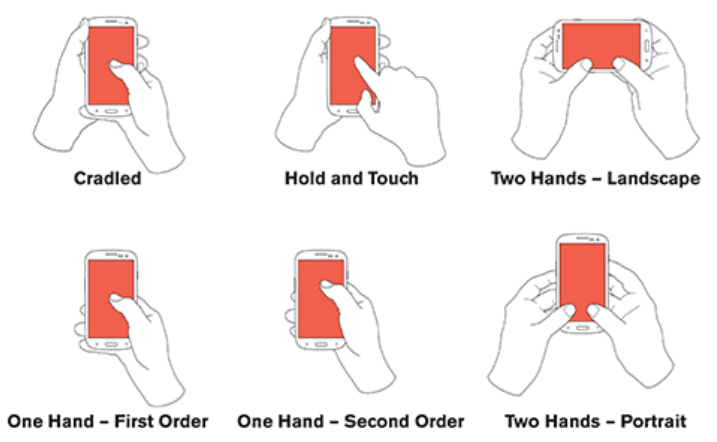
\includegraphics[width=150px]{img/touchInterfaces.png}
        \captionof{figure}{Unterschiedliche Art und Weise wie ein Smartphone bedient wird}
        \label{fig:Smartphone Bedienung}
\end{Figure}
$\rightarrow$ Das hat Auswirkung, wo man welche Elemente platziert

\begin{Figure}
   \centering
    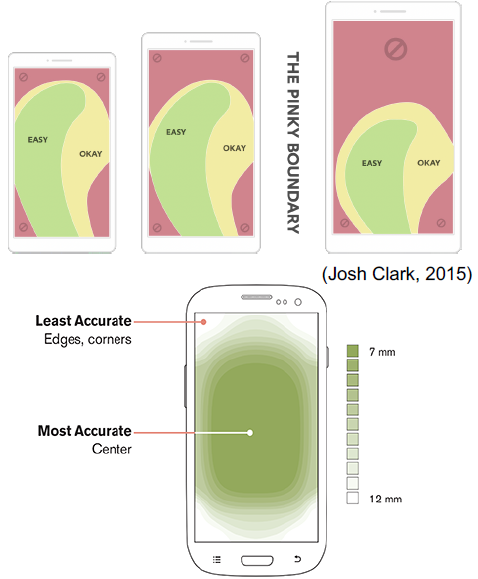
\includegraphics[width=150px]{img/touchInterfacesForRightHand.png}
        \captionof{figure}{Übersicht der Flaechen für Rechtshaender}
        \label{fig:Uebersicht Bedienung fuer Rechtshaender}
\end{Figure}
\begin{itemize}
   \item Platzieren von wichtigen Elemente in den Bereiche 'Easy'
   \item Platzieren von selten Elemente in den Bereich wo man schlecht hinkommt
   \item Platzieren von gefährlichen Aktionen in den Bereich wo man schlecht hinkommt
   \item Man scrollt häufiger als irgendwelche Schaltflächen zu bedienen 
   \item Links und Rechtshänder bedenken
   \item Touch-targets müssen gross genug sein (7-12mm in jede Richtung)
\end{itemize}

Ebenfalls muss man den Ausschluss von Informationen bedenken
\begin{Figure}
   \centering
    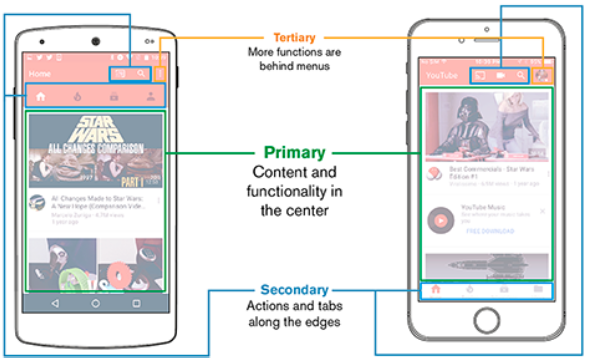
\includegraphics[width=150px]{img/occlusion.png}
        \captionof{figure}{Einteilung der Bereiche}
        \label{fig:Bereichseinteilung}
\end{Figure}
\begin{itemize}
   \item wichtige Inhalte in die primäre Zone (Mitte)
   \item Tendenziell halten die Menschen das Smartphone eher weiter unten, bei sehr grossen Geräten
\end{itemize}

\begin{itemize}
   \item Eine geniale erste Erfahrung mit dem Kunden
   \subitem einfache erste Bedienung
   \subitem kein langwiriger Anmeldeprozess 
   \item Funktionale Animation
   \subitem Jedoch sollte dies nicht übertrieben werde $\rightarrow$ es gibt Personen mit Epilepsie etc. 
   \item Der ganze Service-Prozess überarbeiten, nicht nur die App
   \subitem nicht nur die App testen, sondern der ganze Prozess welcher dazu gehört
   \subitem Push-Notification verhindern 
\end{itemize}

\subsection{Zusammenfassend}
\begin{itemize}
   \item Touch ist nicht präzise
   \item Die User nutzen nur was sie sehen
   \item Telefone sind nicht flach $\rightarrow$ wenn man den Daumen strecken muss, dann bewegt man das Telefon drei dimensional
   \item Tests mit den entsprechenden Personen
\end{itemize}

\section{Styleguides}
Styleguides gibt es für Android, Apple und Windows und definieren wie eine App in etwa auszusehen hat und wie die Interaktionen damit aussehen.\\
Diese dienen als Orientierung, dass man die oben genannten Regeln nicht auswendig wissen. 
$\rightarrow$ auch in Styleguides ist nicht alles perfekt, aus diesem Grund soll beispielsweise die App mit den Nielsen-Regeln überprüft werden

\chapter{Detailed Design of NUIs}

\section{Affordance}
Was zeichnet ein gutes Interaktionselement aus? $\rightarrow$ Affordances (Angebotscharakter)\\
bspw. bei einem Link die unterstrichene Linie\\
\begin{itemize}
   \item Percetible Affordance
   \subitem bspw. unterstrichener Link 
   \item False Affordance
   \subitem bspw. Schaltfläche welche man nicht drücken kann 
   \item Hidden Affordance
   \subitem bspw. Schütteln bei der SBB ab (Niemand kennt diese Funktion)
\end{itemize}

\begin{Figure}
   \centering
    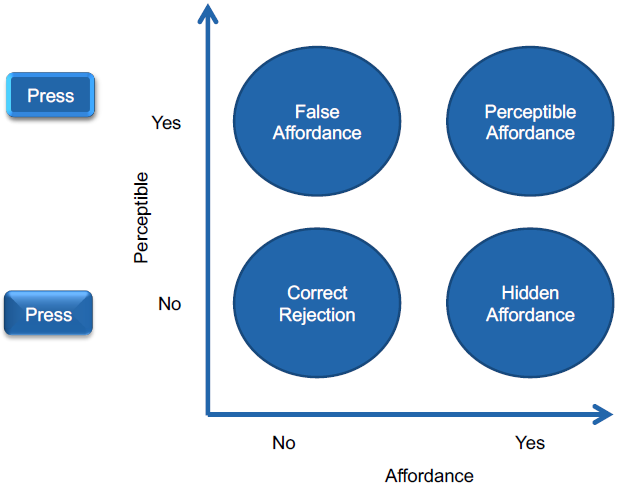
\includegraphics[width=150px]{img/Affordance.png}
        \captionof{figure}{Affordance Eingliederung}
        \label{fig:Affordance Eingliederung}
\end{Figure}

\subsection{Affordance für Gesten}
\begin{itemize}
   \item tap
   \item Slide, Swipe, Fling, Flick
   \item Drag
\end{itemize}

\chapter{App Design}

\section{Prozess}
\begin{enumerate}
   \item Research
   \item Design
   \item User Testing (Usability)
   \item Coding
   \item User Testing (Usability, A/B, Betas)
   \item Publish
\end{enumerate}

\section{Research}
\subsection{Design Consideration}
\begin{itemize}
   \item Context
   \item Purpose
   \item Target Audience
   \item Target Device
\end{itemize}

\subsubsection{Purpose}
\begin{itemize}
   \item Digitaler Assistent für kleine Tasks (Todo, Notizen)
   \item Zeitvertreib
   \item Digital enhancement or support
\end{itemize}

\subsubsection{Target Audience}
\begin{itemize}
   \item Desktop: <Role>
   \item Mobile: <Role>+<Context>
   \item + 'bonus' user groups like impaired people
\end{itemize}

\section{Design Process}
\begin{enumerate}
   \item Sketch
   \item Wireframes
   \item Detail Design
\end{enumerate}

\section{Design for Android}

\subsection{Alternate Layouts}
Sind dafür da, dass man die unterschiedlichen Device-Typen mit der Android-App definieren kann. 

\subsection{px, dp, sp}
\begin{itemize}
   \item elastisches Design ist notwendig
   \item skalierbare Grössen:
   \subitem dp = px * scaling factor
   \subitem sp = dp * user's font size 
   \item für Bilder kann man vektor Grafiken verwenden
\end{itemize}
$\rightarrow$ dp und sp immer verwenden, falls möglich

\subsubsection{Vector vs. Raster Graphics}
\begin{itemize}
   \item Support von vector Grafiken ist nicht all zu gut supported bei Android
   \item Für jeden Bildpunkt wird 3 Bytes gebraucht
\end{itemize}

\subsection{Android Desnity Buckets}
\begin{Figure}
   \centering
    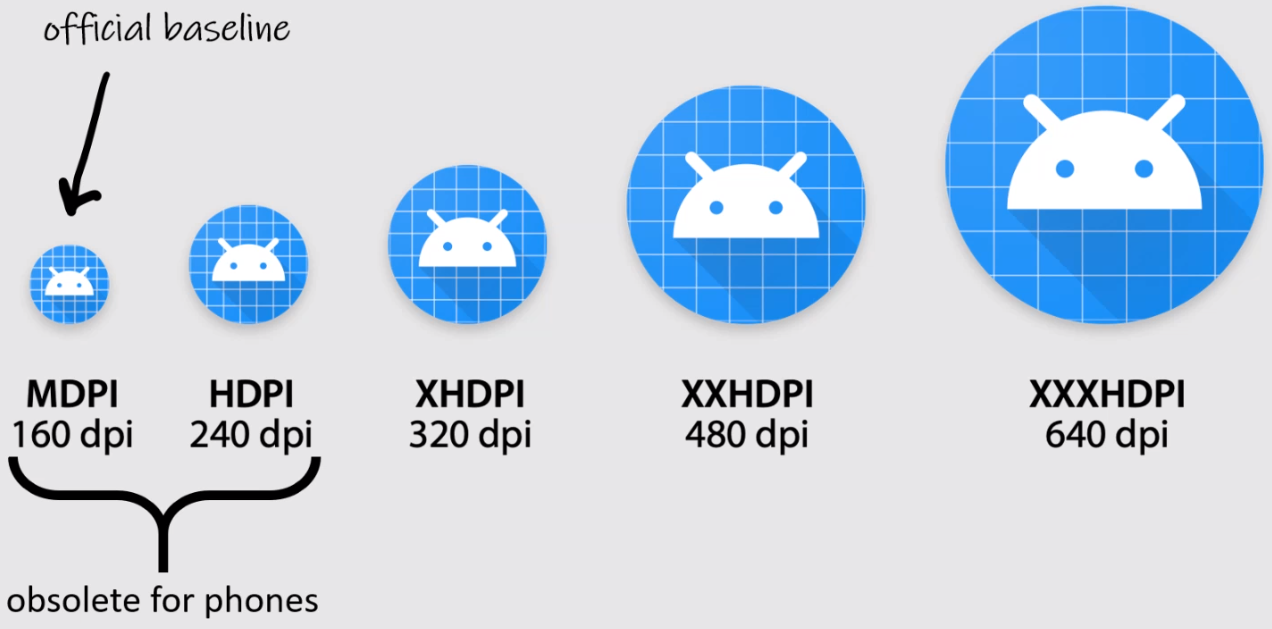
\includegraphics[width=150px]{img/DensityBuckets.png}
        \captionof{figure}{Android Density Buckets}
        \label{fig:Android Density Buckets}
\end{Figure}
$\rightarrow$ auf jedem Gerät ist die Grösse im Vergleich zum Bildschirm gleich gross

\subsection{9-Patch Files}
\begin{itemize}
   \item Ist eine Spezialität von Android, gibts bei IOS nicht
   \item Ist eine Art und Weise wie man Bilder für Android aufbereiten kann
\end{itemize}

\subsection{Was ist klickbar?}
Woran erkenne ich, wenn eine Schaltfläche klickbar ist?
\begin{itemize}
   \item Hervorhebung
   \item Beschriftung
   \item Farbe
   \item Platzierung
\end{itemize}

\section{Material Design}
\begin{itemize}
   \item Ist inspiriert durch die echte Welt
   \item reflektiert diese Belichtung und Schattierung
   \item Manchmal jedoch eher schwierig zu erkennen
\end{itemize}

\subsection{Basic Structure}
\begin{itemize}
   \item Top-Bereich (App-Bar) ist mehr oder weniger fixiert, hier sollte man nicht sonderlich kreativ sein
   \item Jedoch kann man beim Hauptbereich relativ kreativ sein
\end{itemize}

\subsection{Navigation in Android}

\begin{Figure}
   \centering
    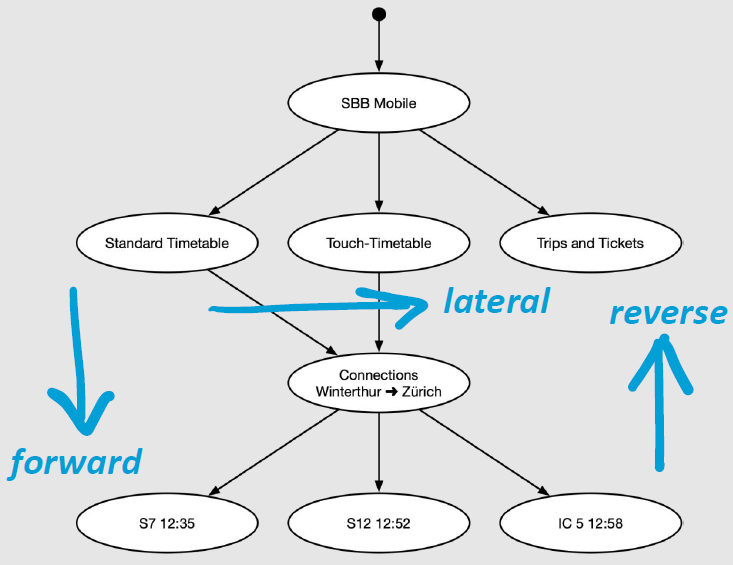
\includegraphics[width=150px]{img/Navigation.png}
        \captionof{figure}{Navigation in Android}
        \label{fig:Navigation in Android}
\end{Figure}

\begin{itemize}
   \item Bottom navigation $\rightarrow$ 2-5 items
   \item Tabs $\rightarrow$ 2-5 items
   \subitem Funktioniert auf jedem Level bspw. auf jedem Level eigene Tabs 
   \item drawer $\rightarrow$ 5-9 items
   \item Springboard $\rightarrow$ 5-9 items $\Rightarrow$ nicht grundsätzlich akzeptiert, muss validiert werden
   \item  Know and unknown $\rightarrow$ 5-9 items $\Rightarrow$ nicht grundsätzlich akzeptiert, muss validiert werden
\end{itemize}

\begin{Figure}
   \centering
    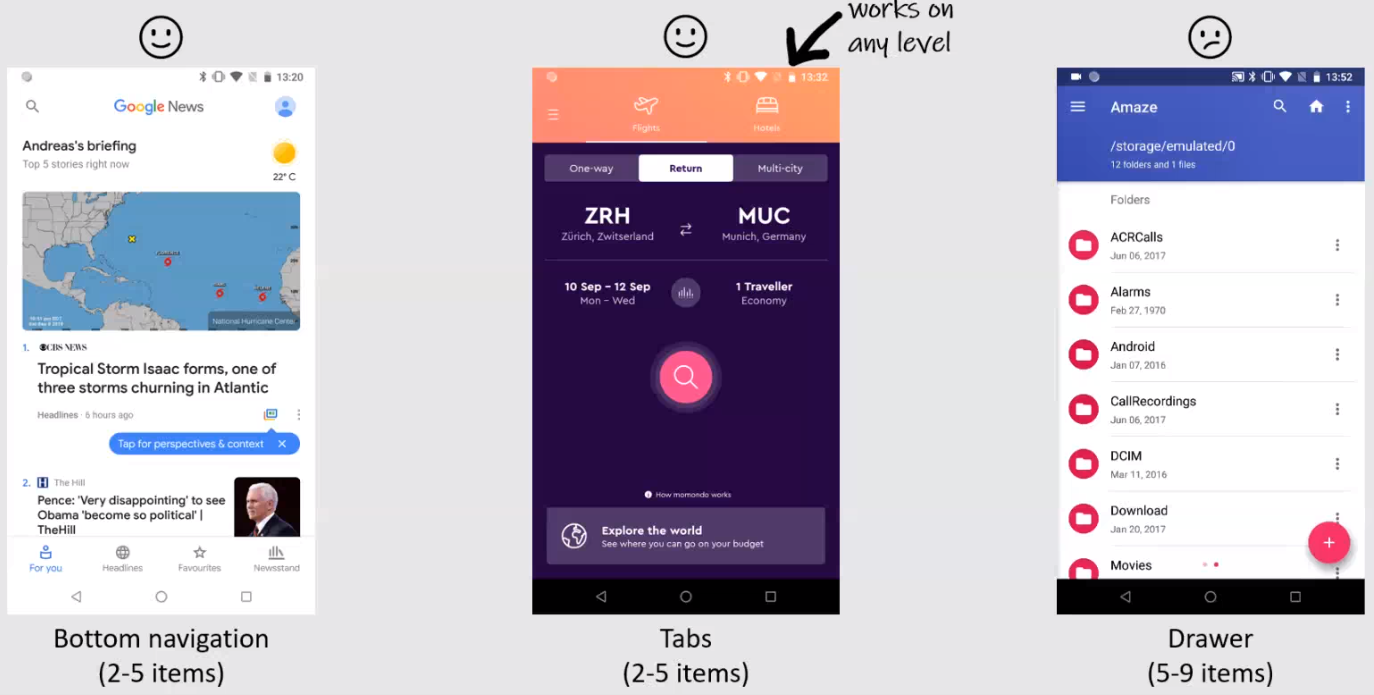
\includegraphics[width=150px]{img/LateralNavigation.png}
        \captionof{figure}{Lateral Navigation in Android}
        \label{fig:Lateral Navigation in Android}
\end{Figure}

\textbf{Was kann man machen, wenn man mehr Elemente hat?}
\begin{itemize}
   \item Informationsarchitektur anpassen
   \item ....
\end{itemize}

\section{Design Empfehlungen}
\begin{itemize}
   \item Alle Screens nach Nielsen überprüfen
   \item an Guidelines halten
   \item Schau was andere machen
   \item gib immer Feedback
   \item Navigation immer ersichtlich
   \item Alle Icons benennen
   \item Farben allein reichen nicht aus
   \item Genügend Kontrast herstellen
   \item genügend grosse und dicke Schriften
   \item accessibility zulassen
   \item 
\end{itemize}

\chapter{App Design mit Kotlin}

\section{Aufbau}
\begin{Figure}
   \centering
    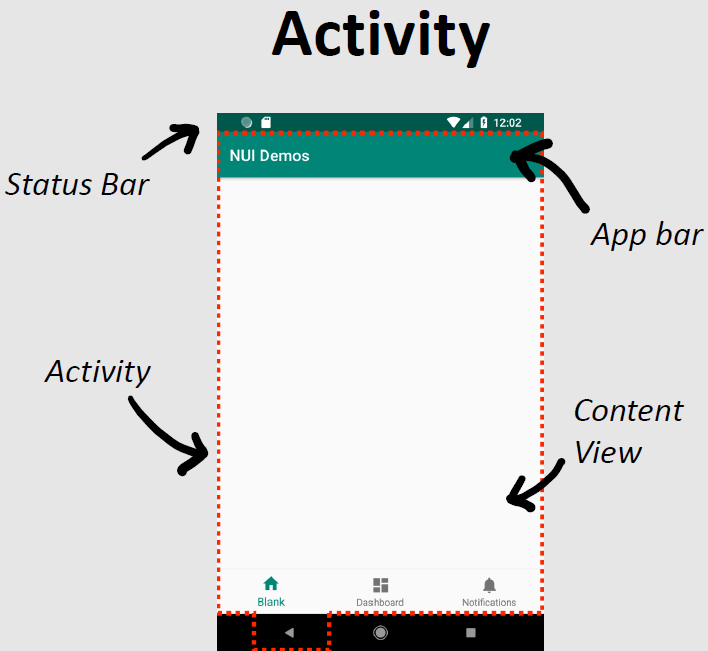
\includegraphics[width=150px]{img/Activity.png}
        \captionof{figure}{Activity dargestellt in roter Linie}
        \label{fig:Activity in Android}
\end{Figure}

\textbf{Fragemente}
\begin{itemize}
   \item Lebt innerhalb der Activity
   \item Für wechselnder Content (tabs, swiping, dialogs)
   \item ermöglicht flexible Layouts
\end{itemize}

\textbf{Views}
\begin{itemize}
   \item Alles was man auf dem Screen sieht ist eine View
   \item Activity und Fragements sind leere Hüllen
\end{itemize}

\section{App Strukturierung}
Möglichkeit
\begin{enumerate}
   \item Mehrere Aktivitäten
   \item 1 Aktivität, viele Fragemente
   \item 1 Aktivität, viele Views $\rightarrow$ heute sehr beliebt bei grossen Teams / Apps
\end{enumerate}



\chapter{Android App Development II}

\section{Threading}
\textbf{UI-Thread:} Sämtliche sind Systeme sind als single Threads abgebildet\\
Dafür Zuständig, dass die Events realisiert werden bzw. Scrollen, Button klicken etc.\\

Nachteil: der UI-Thread kümmert sich immer nur um einen Thread $\rightarrow$ wenn es relativ lange braucht um den Event zu bearbeiten, dann ist die Anwendung so lange blockiert\\

Man hat 16.7ms Zeit den Screen in der App aufzubauen

\section{Fast lists}

\section{Concurrent Programming}


\chapter{Patterns for UIs}

\section{Observer Patterns}
Man hat an diversen Stellen im UI dieselbe Funktionalität. Beispielsweise in Spotify der Pause-Button.\\
das Observer Pattern löst dieses Problem

\begin{Figure}
   \centering
    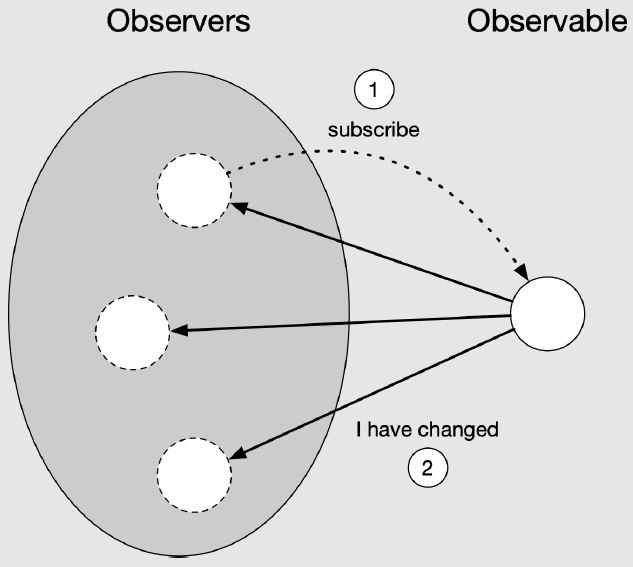
\includegraphics[width=150px]{img/ObserverMechanics.png}
        \captionof{figure}{Der Mechanismus des Observer Pattern}
        \label{fig:Observer Mechanismus}
\end{Figure}
\begin{itemize}
   \item Observable: Quelle
   \item Observer: Subscriben das Observable, welche interessiert an diesem sind
   \item Es ist reactive
   \item Man muss nicht nachfragen, sondern es wird informiert
   \item Gute Entkopplung
\end{itemize}

\begin{Figure}
   \centering
    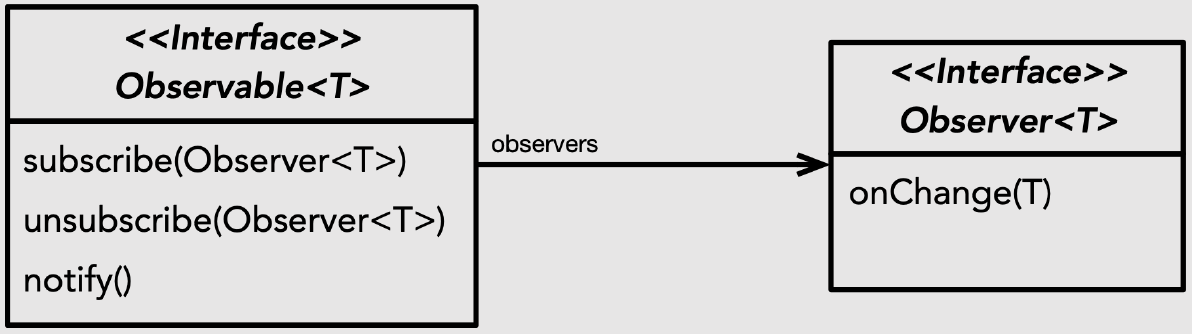
\includegraphics[width=150px]{img/ObserverStructure.png}
        \captionof{figure}{Die Struktur (in UML) des Observer Pattern}
        \label{fig:Observer Struktur}
\end{Figure}

\textbf{Anwendung von Observer}\\
\begin{itemize}
   \item Event Handling - addOnClickListener()
   \item RxJava
   \item EventBus (Guava, Spring)
   \item Data Binding
\end{itemize}

\section{Model View Controller and Friends}

\subsection{Model View Controller}
\begin{itemize}
   \item Ohne Observer gibt es kein MVC
   \item Trennung zwischen Model, View und Controller
\end{itemize}


\begin{Figure}
   \centering
    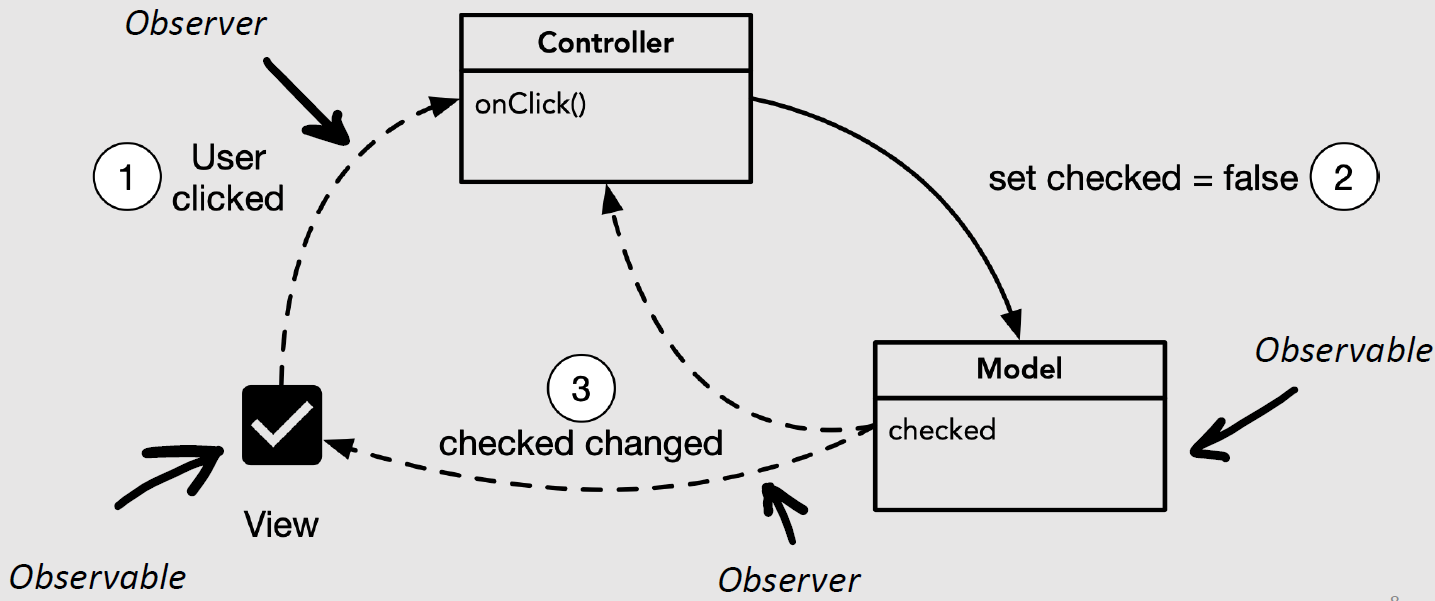
\includegraphics[width=150px]{img/MVC.png}
        \captionof{figure}{MVC Abbildung}
        \label{fig:MVC Abbildung}
\end{Figure}

\begin{Figure}
   \centering
    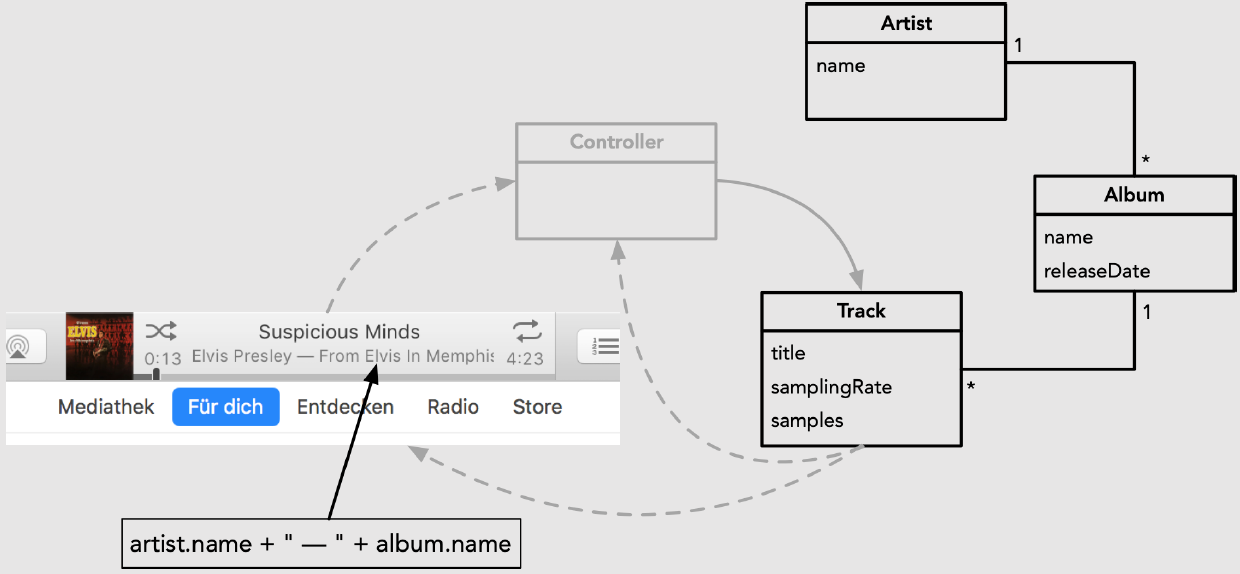
\includegraphics[width=150px]{img/MVCModel.png}
        \captionof{figure}{MVC-Model Abbildung}
        \label{fig:MVC Model Abbildung}
\end{Figure}

\begin{Figure}
   \centering
    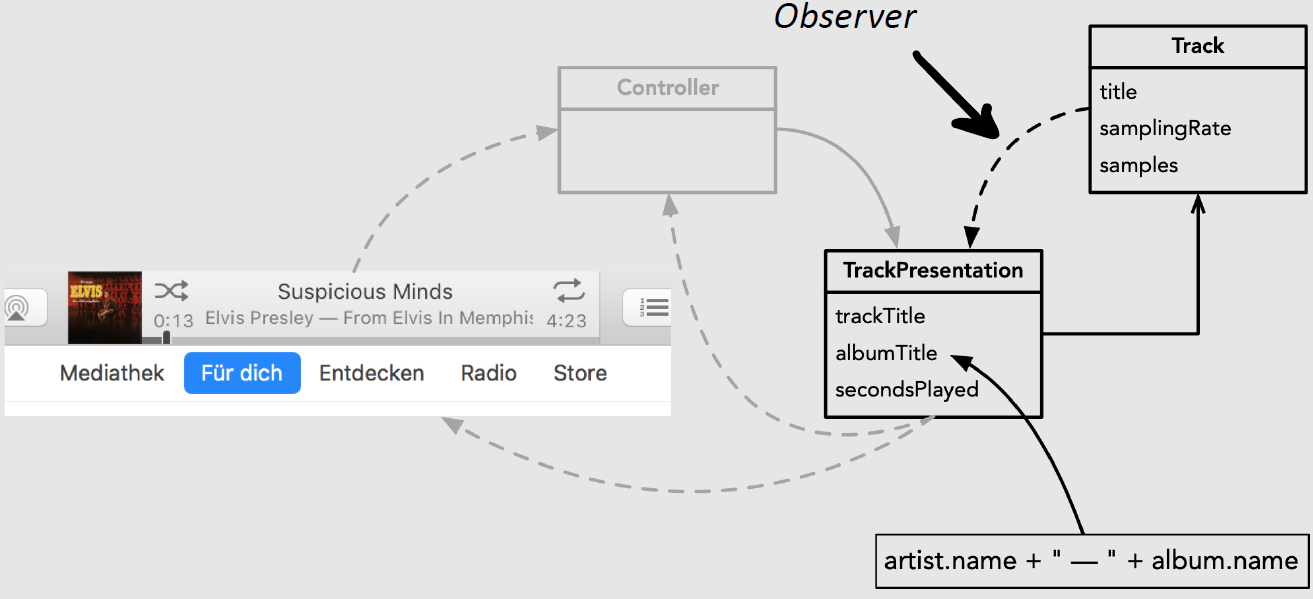
\includegraphics[width=150px]{img/MVCPresentation.png}
        \captionof{figure}{MVC-Presentation Abbildung}
        \label{fig:MVC Presentation Abbildung}
\end{Figure}

\begin{Figure}
   \centering
    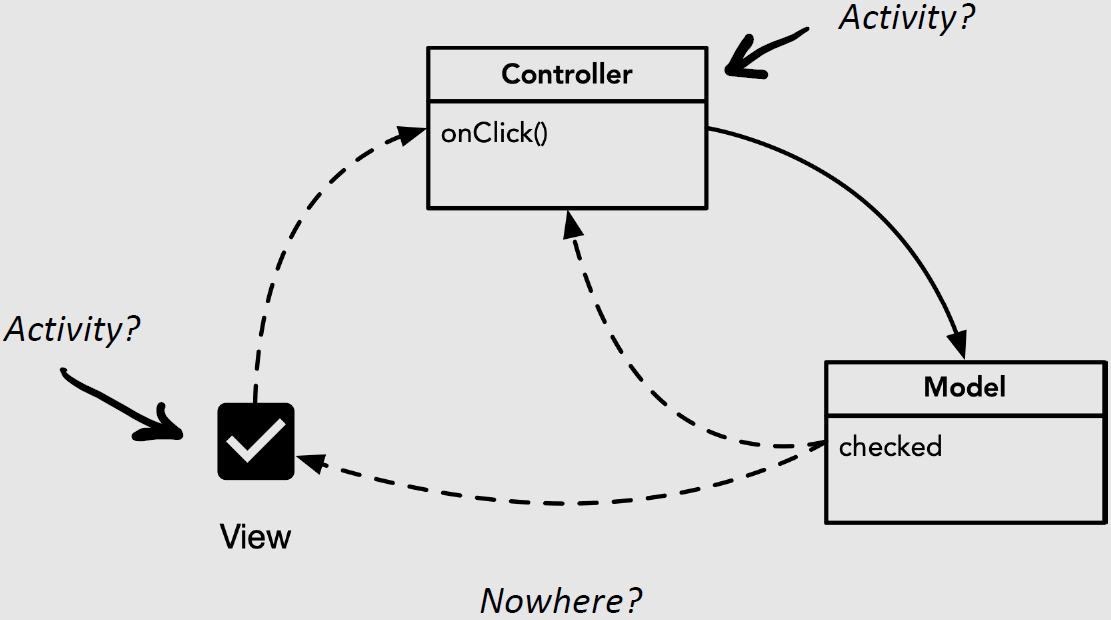
\includegraphics[width=150px]{img/MVCActivity.png}
        \captionof{figure}{MVC-Activity Abbildung}
        \label{fig:MVC Activity Abbildung}
\end{Figure}

\subsection{MVP}
\begin{Figure}
   \centering
    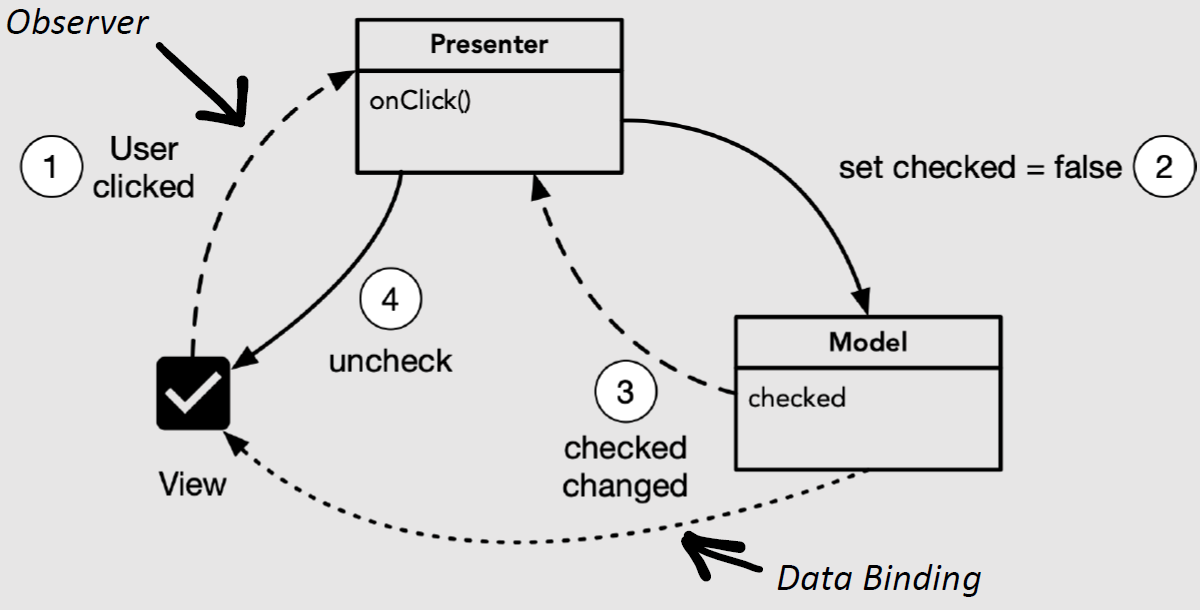
\includegraphics[width=150px]{img/MVP.png}
        \captionof{figure}{MVP Abbildung}
        \label{fig:MVP Abbildung}
\end{Figure}

\begin{Figure}
   \centering
    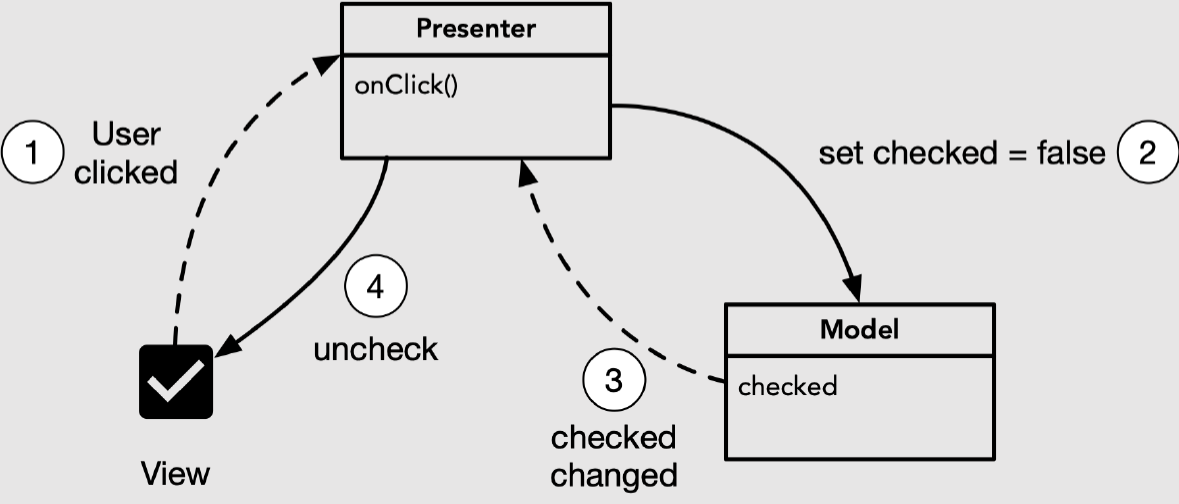
\includegraphics[width=150px]{img/MVPPassiveView.png}
        \captionof{figure}{MVP Passive View Abbildung}
        \label{fig:MVP Passive View Abbildung}
\end{Figure}

\subsection{Model View ViewModel}

\begin{Figure}
   \centering
    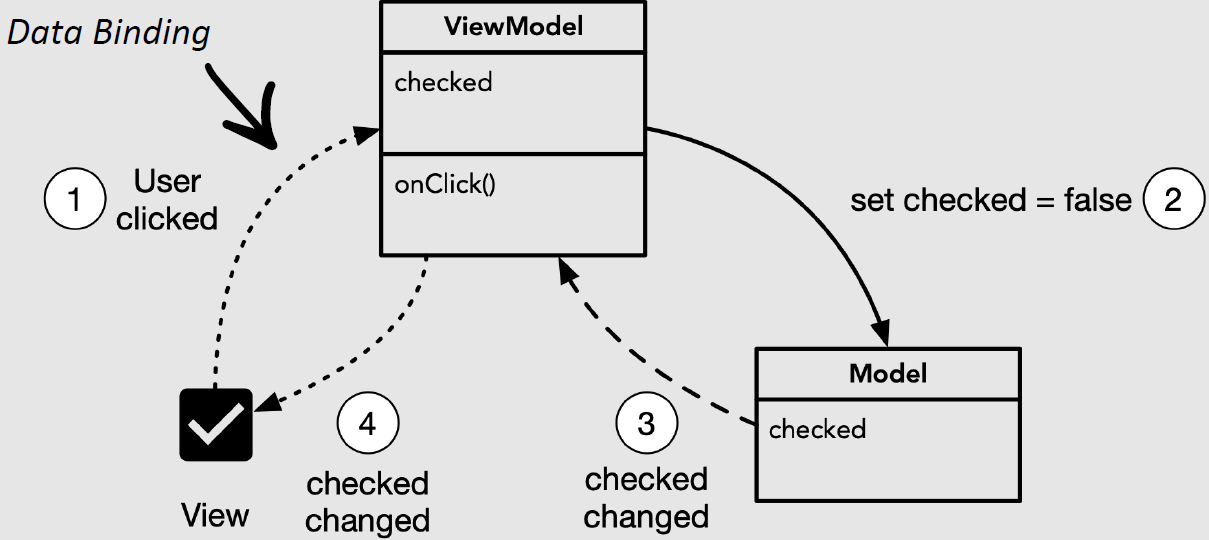
\includegraphics[width=150px]{img/MVVM.png}
        \captionof{figure}{MVVM Abbildung}
        \label{fig:MVVM Abbildung}
\end{Figure}

\section{Chain of Responsibility}
Behandelt sich darum, wer ist verantwortlich einen Event abzuarbeiten

\begin{Figure}
   \centering
    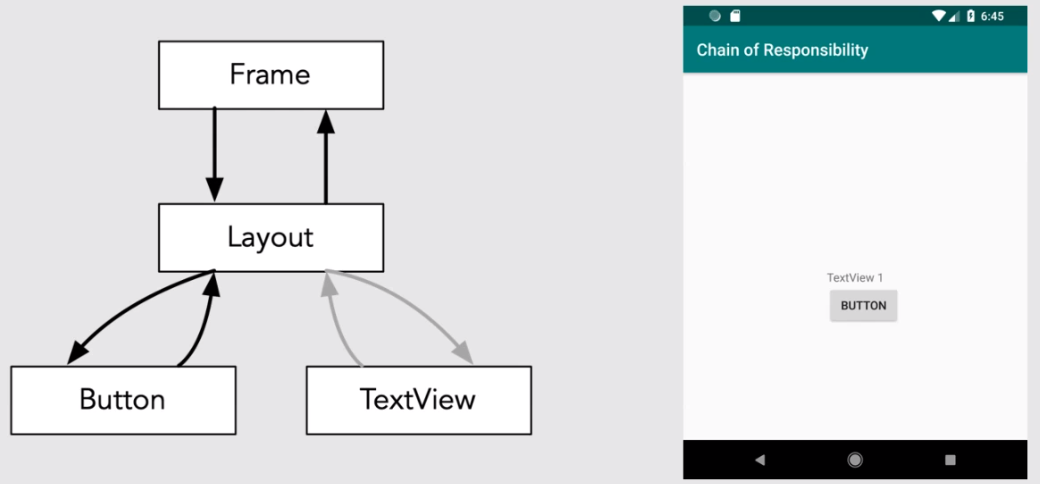
\includegraphics[width=150px]{img/CoR.png}
        \captionof{figure}{Chain of Responsibility}
        \label{fig:Chain of Responsibility}
\end{Figure}
Frame kann nichts damit anfangen $\rightarrow$ Frame fragt Layout, kannst du was damit anfangen? $\rightarrow$ Layout kann ebenfalls nichts damit anfangen $\rightarrow$ Layout fragt Button, kannst du was damit anfangen? $\rightarrow$ Button antwortet, mit ja ich kümmere mich darum\\

\section{Composite}


\chapter{User and Domain Research}
Ist eine der wichtigsten Phase, jedoch gibt es sehr viele Ausreden, weshalb man diese Phase überspringen möchte\\

\section{User}
Unterscheidung wie folgt
\begin{itemize}
   \item Primary
   \subitem brauchen das System häufig und interagieren direkt mit dem System 
   \item Secondary
   \subitem indirekte oder unregelmässige Verwendung des Systems 
   \item Tertiary
   \subitem Sind betroffen von der Einführung des Systems oder beeinflussen den Kauf des Systems 
\end{itemize}

Was wollen wir von den Usern wissen?
\begin{itemize}
   \item Wer sind die User?
   \item Was sind die Arbeiten, Aufgaben und Ziele?
   \item Was ist der Kontext der Arbeit?
   \item Was sind die Bedürfnisse um die Ziele zu erreichen?
   \item Wie sieht die Domänensprache aus
   \item Gibt es Normen (Organisatorische, kulturelle und soziale)
   \item PaintPoints im Workflow
   \item Zusätzlich für mobile Apps relevant
   \subitem Wo wird die App verwendet (Umgebung: Zuhause etc.)
   \subitem Wann wird die App genutzt (Nacht, Tagsüber etc.)
   \subitem Wieso wird die App genutzt (Motivation und Trigger) 
\end{itemize}

Wie geht man dabei vor?
\begin{enumerate}
   \item Domäne lernen (Ziele, Aufgaben, Konzepte, Begriffe)
   \item Absicht definieren
   \item Ressourcen definieren (time, ressources, finanzielle)
   \item Design Research
   \subitem Zieluser (alter, geschlecht, location, beruf, ausbildun, produkterfahrung)
   \subitem research questions to answer
   \subitem research methods
   \subitem roles
   \subitem Equipment to use
   \item Personen rekrutieren und Zeitplan definieren
   \item Research und protokollieren
   \item Diskussion und Interpretation
   \subitem single case analysis / cross case analysis
   \subitem induktiv / dekutiv
   \item Zusammenfassen und dokumentieren (user stories, personas etc.) 
\end{enumerate}

Techniken für user und domain research
\begin{itemize}
   \item Kontextuelle Nachfrage (contextual inquiry)
   \subitem Experte folgt einem User beim Ausüben des Tasks und stellt dabei Fragen
   \subitem Mischung aus contextual interview und direkter Beobachtung
   \subitem Das wird benötigt: Aufnahmegerät, Kamera, Notizbuch und Stift
   \subitem Geeignet für: Fehlerauffindung und Szenarien eruieren
   \item Contextual interview
   \subitem vor Ort 
   \subitem Klassifiziert nach: strukturiert(geschlossene Fragen), halbstrukturiert(geschlossene und offene Fragen), nicht-strukturiert (keine vorbereiteten Fragen) 
   \item Interviews
   \subitem seperates Kapitel 
   \item Direkte oder indirekte Beobachtungen
   \item Fokusgruppen / Workshops
   \item Befragungen 
   \item Umfragen
   \item Desktop research $\rightarrow$ studying documentation, konkurrenz
\end{itemize}

\begin{Figure}
   \centering
    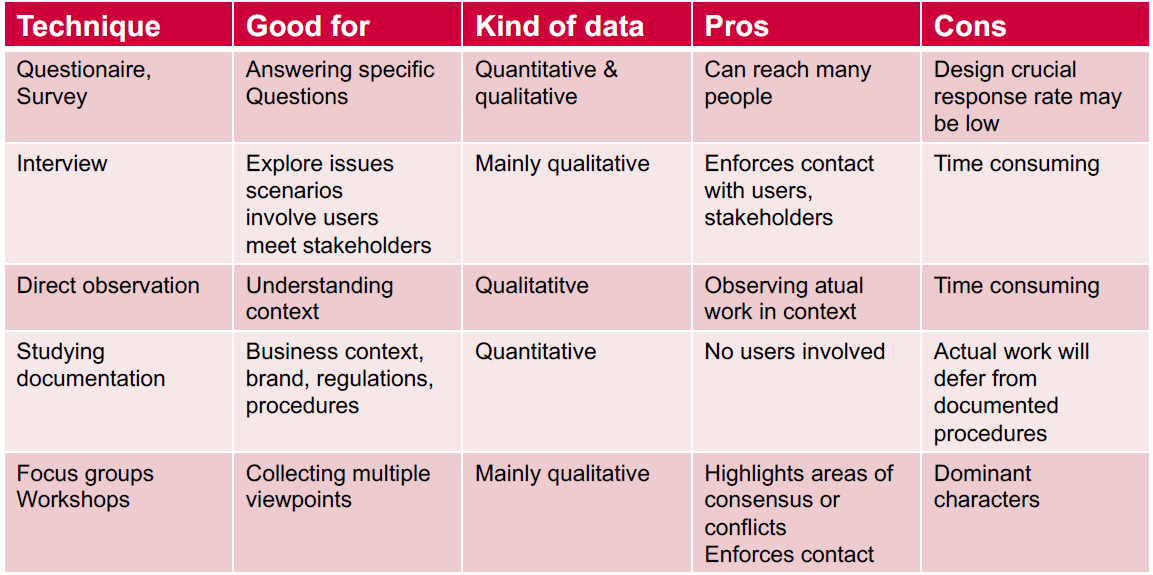
\includegraphics[width=150px]{img/OverviewTechniques.png}
        \captionof{figure}{Übersicht der Techniken}
        \label{fig:Übersicht der Techniken}
\end{Figure}

\subsection{Interview}
Planung:
\begin{itemize}
   \item User-Rollen identifizieren
   \item Bestimmen der mind. Anzahl an Interviewpartner pro Rolle
   \item Für jeden Faktor der das User-Verhalten betrifft, soll es mit der Anzahl unterschiedlichen Gruppen multipliziert werden
   \item Anzahl Interview herunterbrechen
   \item Einplanen, dass es gewisse No-Shows geben wird
   \item Rekrutierung und Planung kann bis zu 2-4 Wochen gehen
\end{itemize}

Wie?
\begin{itemize}
   \item Offene Fragestellung (Wer, Was, Wo, Wieso, wann, wie?)
   \item Es sollte mehr eine Konversation sein
   \item Sympathisch und nicht verurteiltend
   \item Sei der "Lernende" und nicht der "Experte"
   \item naive Frage stellen
   \item Die Personen sollen die Sachen zeigen
   \item Frage nach spezifischen Stories
   \item Falls etwas relevantes vorkommt oder so aussieht, nachfragen
   \item vom aktuellen Zustand zum Problem
   \item auf inkonsistenz achten
   \item gestik und mimik beachten
   \item 30-60 min pro Interview inkl. 30min nachbearbeitung
\end{itemize}

Struktur:
\begin{itemize}
   \item Introduction
   \item Warmup
   \item Main Session
   \item Cool-off period
   \item closing
\end{itemize}

\chapter{Menschliche Wahrnehmung}

\section{Das Menschliche Wahrnehmungssystem}

Die 5 Sinne 
\begin{itemize}
   \item Sehen (80\% der Informationen)
   \item Hören (15\% der Informationen)
   \item Tastsinn
   \item Geruchssinn
   \item Geschmacksinn
\end{itemize}

Die Sensorik ist ein kurzzeit-Gedächnis und ist im Sinne einer FIFO-Queue

\begin{Figure}
   \centering
    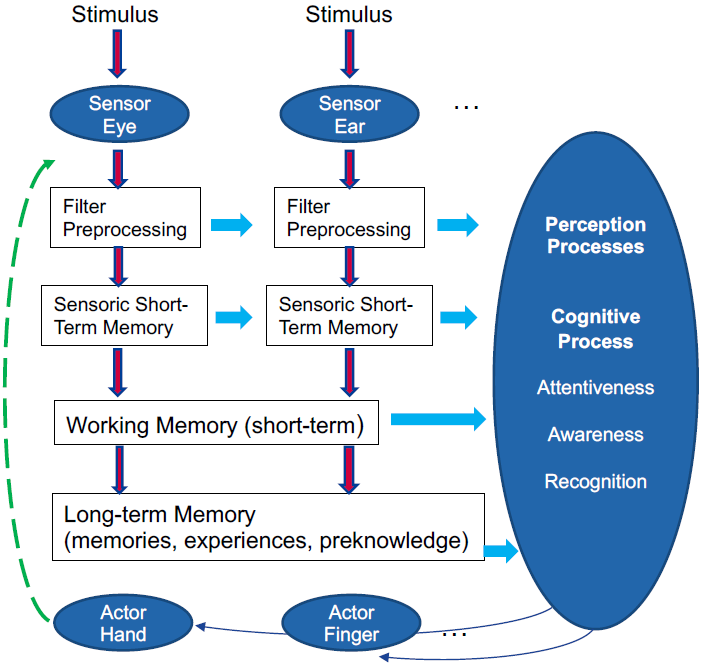
\includegraphics[width=150px]{img/HumanRecognitionSystem.png}
        \captionof{figure}{Abbildung des Ablaufs der Wahrnehmung eines Menschens}
        \label{fig:Abbildung des Ablaufs der Wahrnehmung eines Menschens}
\end{Figure}

\subsection{Sehen}
Das Menschliche Auge:
\begin{itemize}
   \item Iris, Pupille
   \item Retina (Netzhaut) enthält die visuellen Rezeptoren
   \item Macula (gelber Fleck)
   \item Fovea (Sehgrube) $\rightarrow$ Ort grösster Sehschärfe
   \item Blinder Fleck $\rightarrow$ Hier verlassen die Nerven das Augen, entsprechend keine Rezeptoren
\end{itemize}
\begin{Figure}
   \centering
    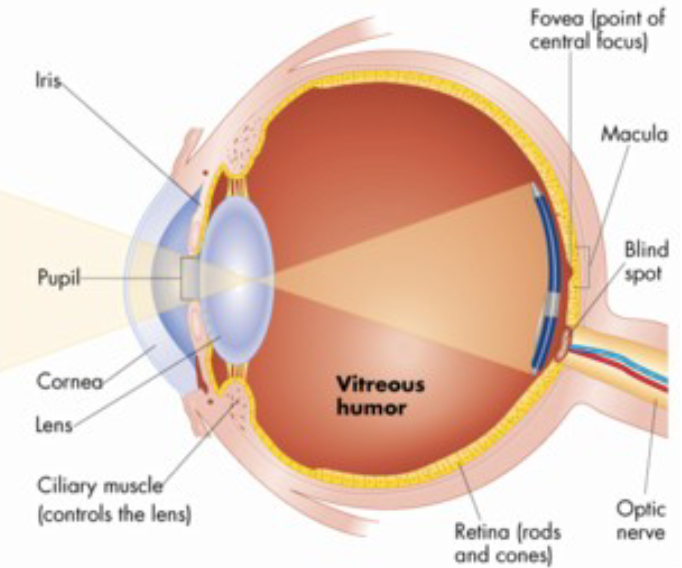
\includegraphics[width=150px]{img/Auge.png}
        \captionof{figure}{Abbildung des menschlichen Auge}
        \label{fig:Abbildung des menschlichen Auge}
\end{Figure}

\subsubsection{Netzhaut}
Hat zwei unterschiedliche Typen von Rezeptoren
\begin{itemize}
   \item Zäpfchen-Zellen
   \subitem L(rot), M(grün), S(blau)
   \subitem für das farbliche Sehen
   \subitem Hauptsächlich in der Macula
   \subitem  Nur in Fovea 
   \item Stäbchen-Zellen
   \subitem Für das Schwarz/weiss Sehen
   \subitem 20mal mehr als Zäpfchen
   \subitem Rest der Netzhaut
   \subitem ca. 200-250 grautöne
\end{itemize}

\begin{Figure}
   \centering
    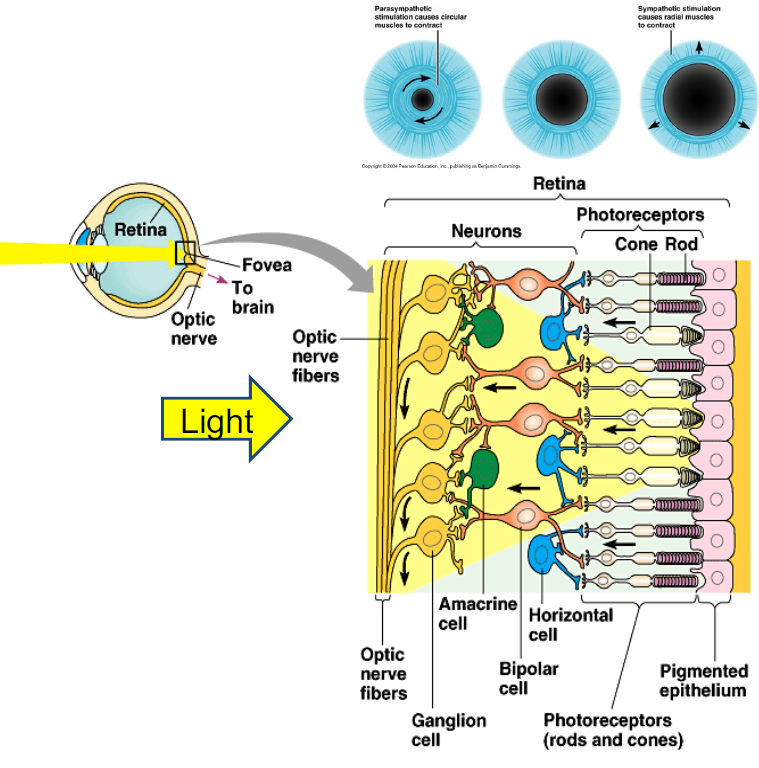
\includegraphics[width=150px]{img/Retina.png}
        \captionof{figure}{Abbildung der Netzhaut}
        \label{fig:Abbildung der Netzhaut}
\end{Figure}

\subsubsection{Farbblindheit}
\begin{itemize}
   \item Protanopie (red-blindness)
   \subitem kann nur schwer zwischen rot, grün, gelb und braun unterscheiden 
   \item Deuteranopie (green-blindness)
   \subitem kann nur schwer zwischen rot, grün, gelb und braun unterscheiden 
   \item tritanopie (blue-blindness)
   \subitem kann nur schwer rot von orange, blau von grün, etc. unterscheiden 
\end{itemize}

\subsubsection{dynamische Sicht}
Bei mehr als 22Bilder pro Sekunde nimmt das Auge dies als dynamische Bewegung auf $\rightarrow$ Film

\subsubsection{Tiefenwahrnehmung}
tbd

\subsection{Hören}
Der Gehörsinn ist für das GUI nur von sekundärer Relevanz, jedoch für mobile interaktionen elementar. \\

Das Sprechen basiert auf Schallwellen, welche von unserem Gehör aufgenommen wird. Diese Schallwellen werden in Schallpegel (dB) gemessen

evtl noch weiter ausführen

\section{menschlicher Verstand}

\subsection{Kurzzeitgedächnis}
\begin{itemize}
   \item Sensorischer Speicher
   \subitem Speichert Sensorsignale im FIFO-Prinzip für ca. eine Sekunde
   \item Arbeitsspeicher
   \subitem extrahiert Dinge und Objekte (bspw. analoge Uhr $\rightarrow$ ablesen der Uhrzeit)
   \subitem speichert die Dinge auf welche mir uns aktuell fokussieren
   \subitem definiert die Aufmerksamkeit, Kontext und Realität
   \subitem kann nicht geteilt werden
   \subitem Kapazität ist limitert (ca. 7 +/- 2 Dinge / Stücke)
\end{itemize}

\subsubsection{Aufmerksamkeit}
\begin{itemize}
   \item ist durch das Kurzzeitgedächnis bestimmt und limitiert
   \item Menschen können verschiedene Dinge gleichzeitig ausführen (vor allem Frauen)
   \subitem Jedoch können wir uns \textbf{nur auf einen einzigen Task gleichzeitig konzentrieren} $\rightarrow$ die andere Dinge müssen automatisch erledigt werden bspw. Autofahren, zuhören, Fahrrad fahren 
\end{itemize}
$\Rightarrow$ Konsequenzen für das UI Design
\begin{itemize}
   \item Die Interaktion mit dem UI sollte so einfach wie notwendig ausfallen, dass dies für (regelmässige Anwender) automatisch passiert
   \item Die Benutzer konzentrieren sich auf die Aufgabe, welche erledigt werden muss, nicht auf die Interaktion mit dem UI
\end{itemize}

\subsection{Langzeitgedächnis}
Hier befindet sich alles was wir bis anhin in unserem Leben gelernt haben.\\s

\textbf{ACT-R Model}
\begin{itemize}
   \item deklaratives Modell
   \subitem Fakten, Daten
   \subitem Konzepte (Wörter, Grammatikregeln, Gefühle, Geschmäcke)
   \item kognitive Unstimmigkeit
   \subitem gewisse Objekte kommen nicht im gewohnten Kontext und sind dadurch nicht eindeutig zu identifizieren  
   \item produktiver Speicher
   \subitem Fähigkeiten (motorische Fähigkeiten bspw. Skifahren oder Autofahren)
   \subitem Automatismen (werden in gewissen Situationen getriggert und automatisch ausgeführt, wozu es keine Aufmerksamkeit braucht)
   \item Tasks 
\end{itemize}
$\Rightarrow$ Wichtig für GUI-Design: Sequence of steps for the same action should always be the same (consistency)

\subsection{Mental Model}
\begin{itemize}
   \item Menschliches Model der Realität
   \item Speichert Konzepte (Nomen) und Assoziationen (Nomen, Attribute, Aktivitäten)
   \item Assoziationen
   \subitem Verbindet neue Fakten und Features mit bestehenden Konzepten
   \subitem Bessere Erinnerung
   \item sind sehr anpassungsfähig
\end{itemize}

\subsubsection{Mismatch}
If the systems UI does not match the actual users mental model, interaction gets very difficult!

\textbf{Designer}
\begin{itemize}
   \item Entwickelt ein mental model des Problems (domain model)
   \item Entwickelt das System und die UI nach dem erstellen Model
\end{itemize}

\textbf{System}
\begin{itemize}
   \item Stellt ein Bild des Systemverhaltens durch die UI dar 
   \item Basiert auf dem Mental Model des Designers
\end{itemize}

\textbf{Users}
\begin{itemize}
   \item Erstellt das Mental Model aufgrund von
   \subitem seiner aktuellen Erfahrungen und seines Wissens
   \subitem geliefertes Systembild
   \subitem interaktionen mit dem System 
\end{itemize}

\textbf{User Centered Design}
\begin{enumerate}
   \item User Research
   \subitem Probiert herauszufinden, wie das mentale model der User beim erstmaligen Verwenden des Systems aussieht 
   \item Design System and UI
   \subitem Welches das Problem löst
   \subitem Stelt die UI einem User zur Verfügung 
\end{enumerate}

\subsection{Erfahrung}
\begin{itemize}
   \item Summe des Wissens
   \item Automatismen
   \item MentalModel
   \item Zwei extreme Ausprägungen
\end{itemize}

\textbf{Experts}
\begin{itemize}
   \item Viel Wissen und Automatismen
   \item Wissen ist oftmals implizit
   \item Kann sich voll auf die Lösung des Problems konzentrieren
   \item sehr effizient
\end{itemize}

\textbf{Beginner}
\begin{itemize}
   \item Keine Erfahrung
   \item Braucht einfache Fakten und Regeln
   \item Müssen zuerst ihr eigenes mentale Modell der Applikation entwickeln
   \item Müssen sich nicht nur auf die Lösung konzentrieren, sondern auch auf die Aufgabe und Interaktionen
   \item Braucht wesentlich mehr Zeit für die Aufgabe
\end{itemize}

\textbf{Normal User}
\begin{itemize}
   \item Oft ein gewöhnlicher User
   \item Have to recall / rebuild mental model of the system behaviour each time
\end{itemize}

\subsection{Lerntypen}
Die Systeme sollten die User unterstützen im Lernen des Programms, dabei sollte man beachten, dass es unterschiedliche Lerntypen gibt (Sehen, hören, machen, sprechen)\\
Das Lernen wird durch folgende Punkte unterstützt:
\begin{itemize}
   \item Neue mental models werden von existierenden abgeleitet
   \item Metaphern (bspw. Papierkorb)
   \item Schrittweise zusammenführen von neuem mit bestehenden Wissen
   \item Berücksichtigen der Lerntypen
\end{itemize}

\section{Menschliche Erwartungen}
Erfahrung führt zu Erwartungen\\
Das Kano-Modell führt zur Unterstützung der Anforderungne

\section{Menschliches Handeln}
tbd



\chapter{Web Accessability}
\begin{itemize}
   \item ca. 10-15 Prozent Weltweit sind behindert
   \item ca. 300k haben eine Sehbehinderung in der Schweiz
   \item ca. 500k haben eine Gehörbehinderung
\end{itemize}

\section{WCAG}
\begin{itemize}
   \item WCAG: Web Content Accessability Guidelines
   \item in 4 Prinzipien
   \subitem Perceivable
   \subitem Operable
   \subitem Understandable
   \subitem Robust
   \item Dabei gibt es Erfolgskriterien A, AA, AAA, AAAA 
\end{itemize}

\section{UAAG}
\begin{itemize}
   \item User Agent Accessability Guidelines
   \item Guidelines on how to make user agents accessible
   \item User agents include browsers, browsers extentions
\end{itemize}

\section{ATAG}
\begin{itemize}
   \item Authoring Tool accessibility Guidelines
   \item Guidlines on how to make authoring tools such as code editors accessible
   \item Lowers the barrier and provide support for people with disabilities to create more accessible Web content
\end{itemize}

\section{ARIA}
\begin{itemize}
   \item Accesible Rich Internet Applications
   \item A specification to make Web content more accessible to people with disabilites
   \item Especially helpful for dynamic content and advanced user interface controls developed using JavaScript
   \item ARIA stellt verschiedene ROllen zur Verfügung (bspw. Header, main content, navigation, footer)
\end{itemize}


\chapter{Code-Snippets Android}

\section{Material Design as Library}
\begin{Figure}
   \centering
    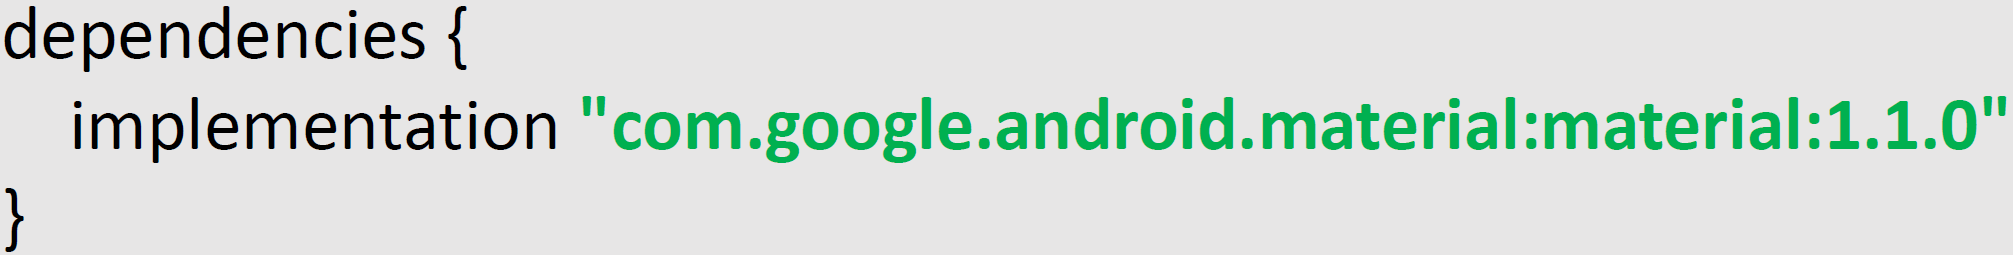
\includegraphics[width=300px]{img/MDaL.png}
        \captionof{figure}{Code Snippet Material Design Dependency}
        \label{fig:Code Snippet Material Design Dependency}
\end{Figure}

\section{item Layout}
\begin{Figure}
   \centering
    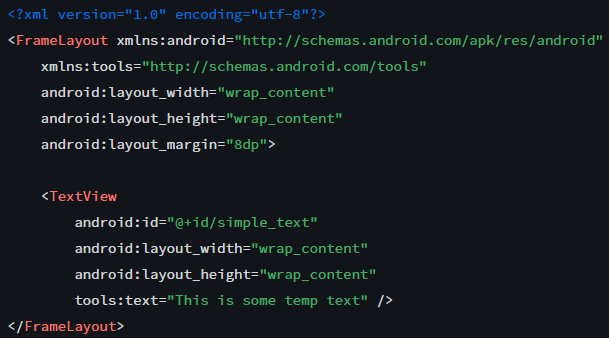
\includegraphics[width=300px]{img/itemLayout.png}
        \captionof{figure}{Code Snippet itemLayout}
        \label{fig:Code Snippet Main Activity itemLayout}
\end{Figure}

\section{Kotlin Main Activity}
\begin{Figure}
   \centering
    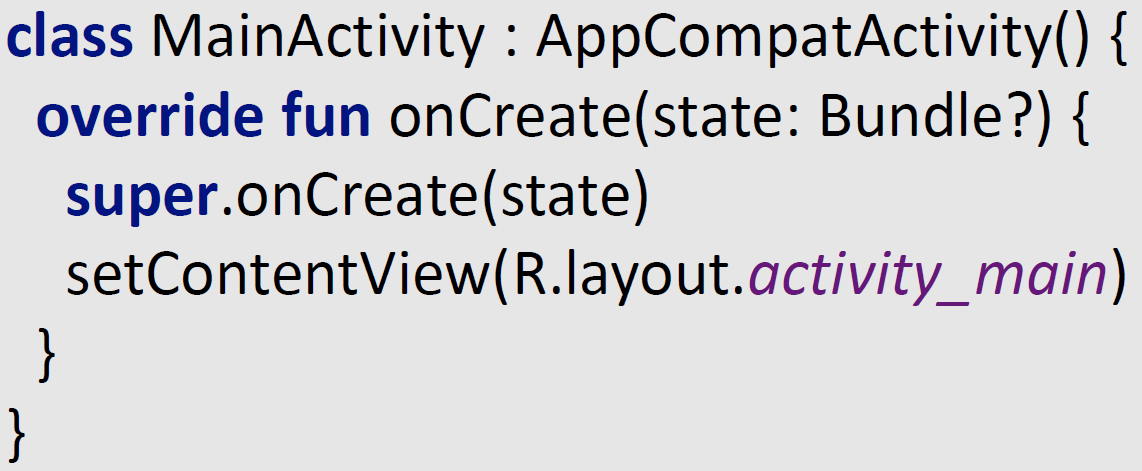
\includegraphics[width=300px]{img/KotlinMainActivity.png}
        \captionof{figure}{Code Snippet Main Activity in Kotlin}
        \label{fig:Code Snippet Main Activity in Kotlin}
\end{Figure}

\begin{Figure}
   \centering
    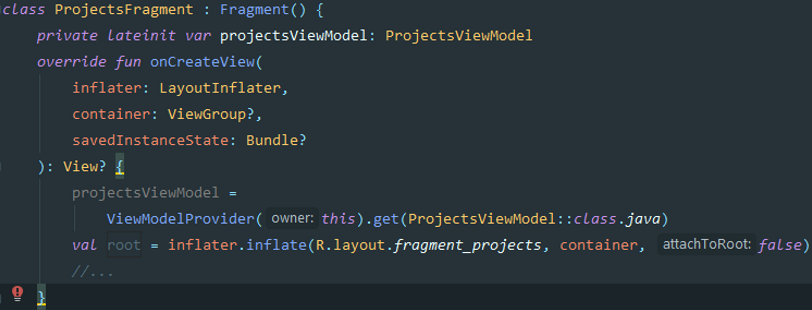
\includegraphics[width=300px]{img/layoutInflater.png}
        \captionof{figure}{Code Snippet Using LayoutInflater to set view for fragment}
        \label{fig:Code Snippet Using LayoutInflater to set view for fragment}
\end{Figure}


\section{Activity Lifecycle}
\href{https://developer.android.com/guide/components/activities/activity-lifecycle#kotlin}{Android Documentation}

\begin{Figure}
   \centering
    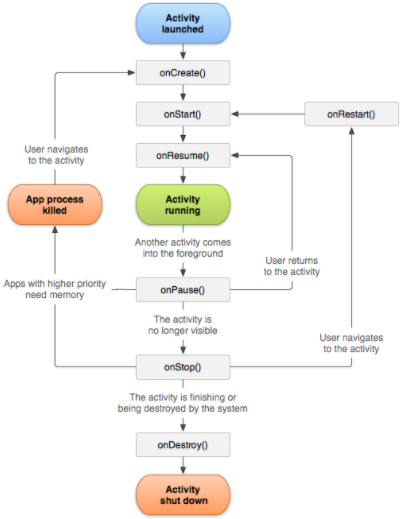
\includegraphics[width=300px]{img/ActivityLifecycle.png}
        \captionof{figure}{Activity Lifecycle }
        \label{fig:Activity Lifecycle}
\end{Figure}
\subsection{onCreate()}
\begin{Figure}
   \centering
    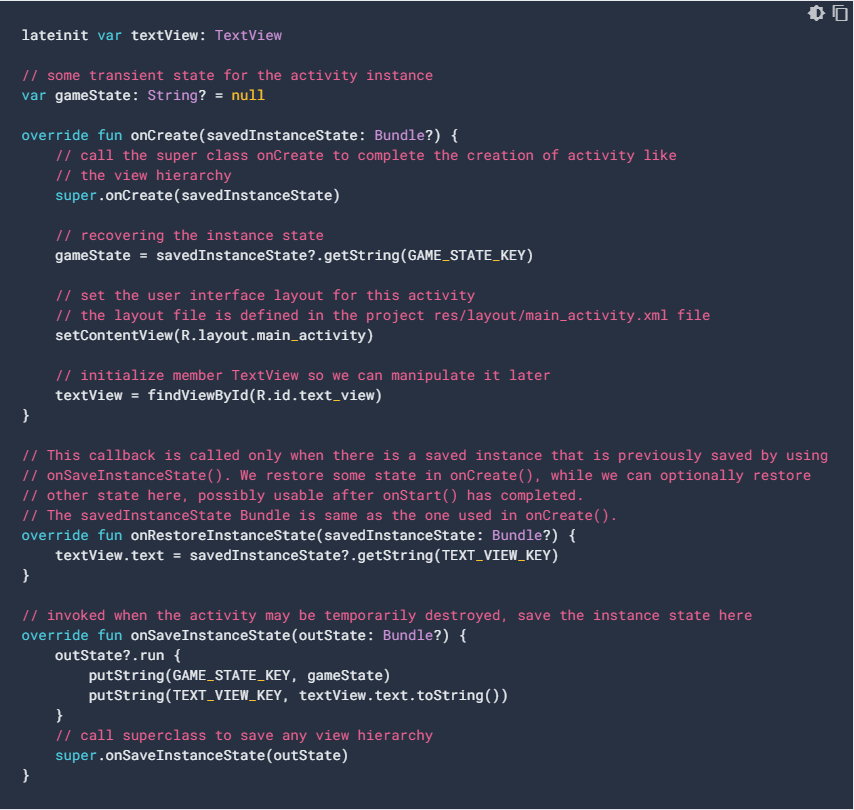
\includegraphics[width=300px]{img/onCreate.png}
        \captionof{figure}{Code Snippet Create Activity Lifecycle onCreate()}
        \label{fig:Code Snippet Create Activity Lifecycle onCreate()}
\end{Figure}

\subsection{onResume()}
\begin{Figure}
   \centering
    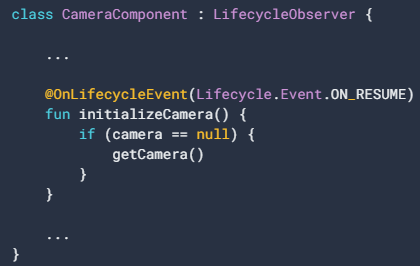
\includegraphics[width=300px]{img/onResume.png}
        \captionof{figure}{Code Snippet Create Activity Lifecycle onResume()}
        \label{fig:Code Snippet Create Activity Lifecycle onResume()}
\end{Figure}

\subsection{onPause()}
\begin{Figure}
   \centering
    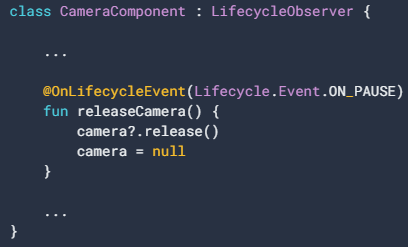
\includegraphics[width=300px]{img/onPause.png}
        \captionof{figure}{Code Snippet Create Activity Lifecycle onPause()}
        \label{fig:Code Snippet Create Activity Lifecycle onPause()}
\end{Figure}

\subsection{onStop()}
\begin{Figure}
   \centering
    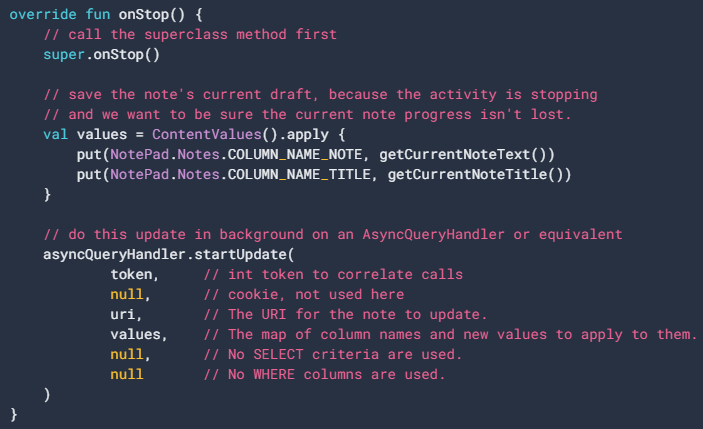
\includegraphics[width=300px]{img/onStop.png}
        \captionof{figure}{Code Snippet Create Activity Lifecycle onStop()}
        \label{fig:Code Snippet Create Activity Lifecycle onStop()}
\end{Figure}

\subsection{Preserving Instance State}
\begin{Figure}
   \centering
    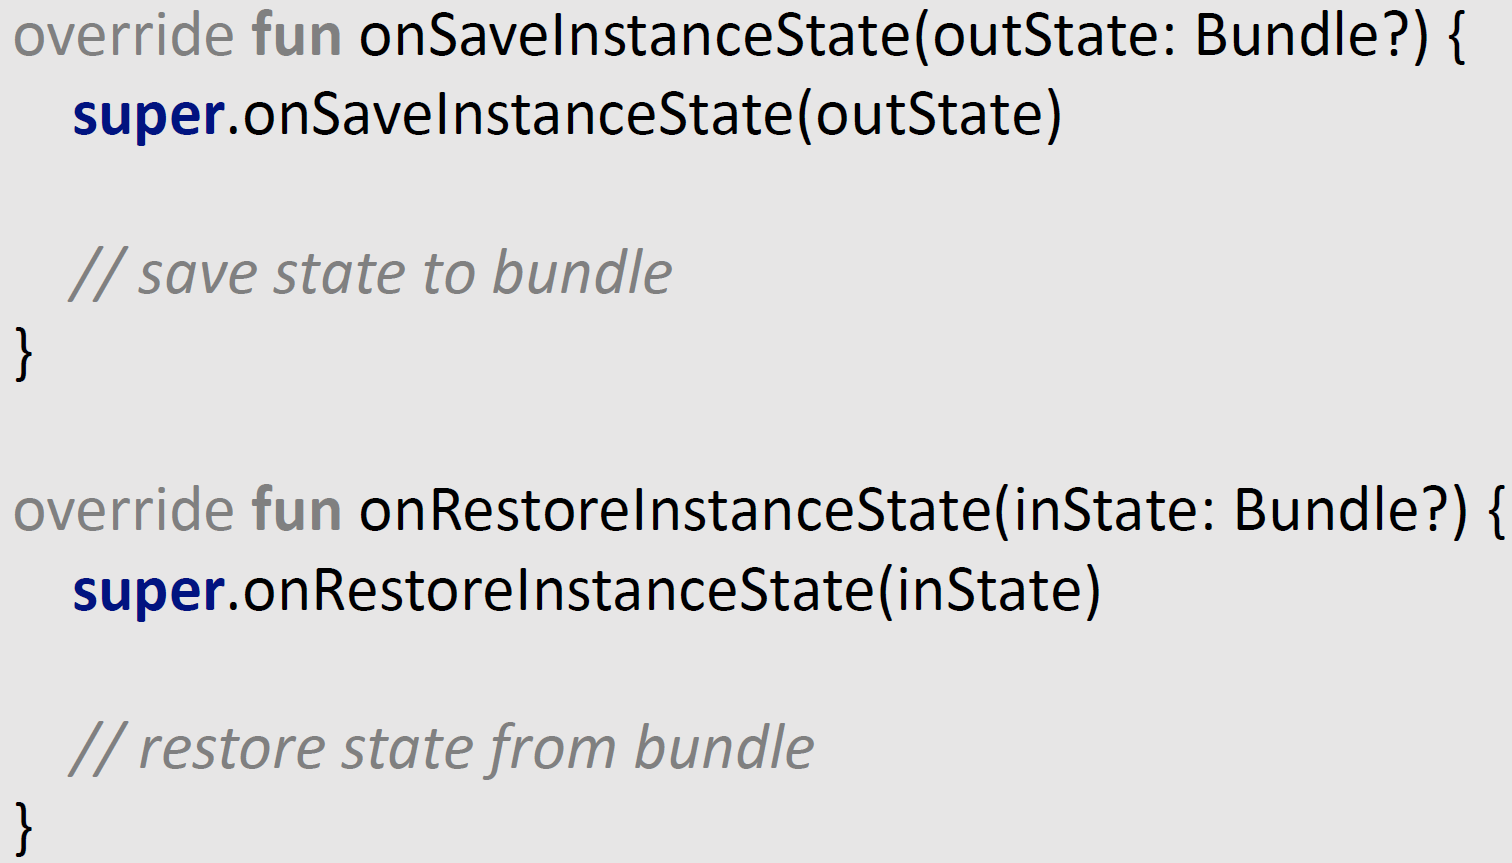
\includegraphics[width=300px]{img/PreservingInstanceState.png}
        \captionof{figure}{Code Snippet Preserving Instance State}
        \label{fig:Code Snippet Preserving Instance State}
\end{Figure}

\section{Intents}
\subsection{Creating Intents}
\begin{Figure}
   \centering
    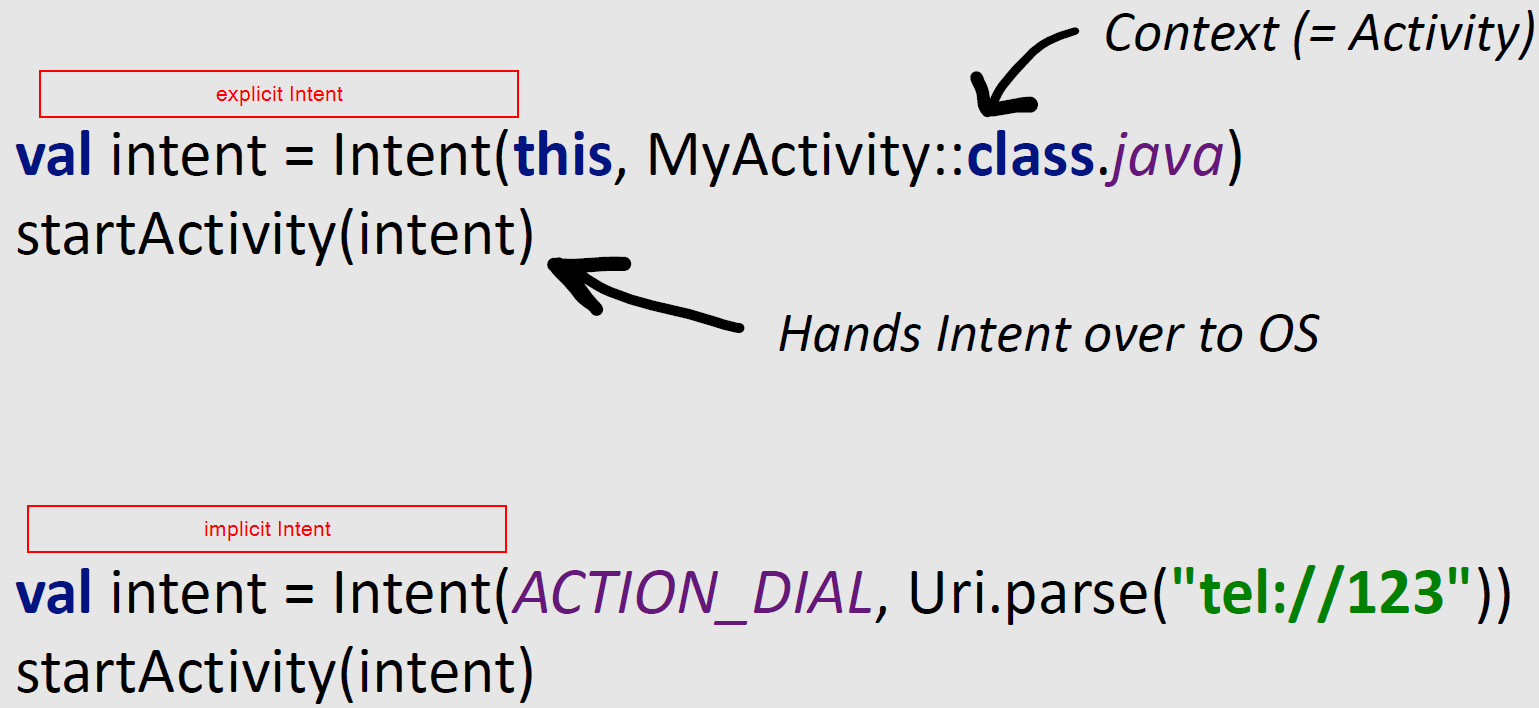
\includegraphics[width=300px]{img/creatingIntents.png}
        \captionof{figure}{Code Snippet Creating explicit and implicit intents}
        \label{fig:Code Snippet Creating explicit and implicit intents}
\end{Figure}

\subsection{Passing Arguments}
\begin{Figure}
   \centering
    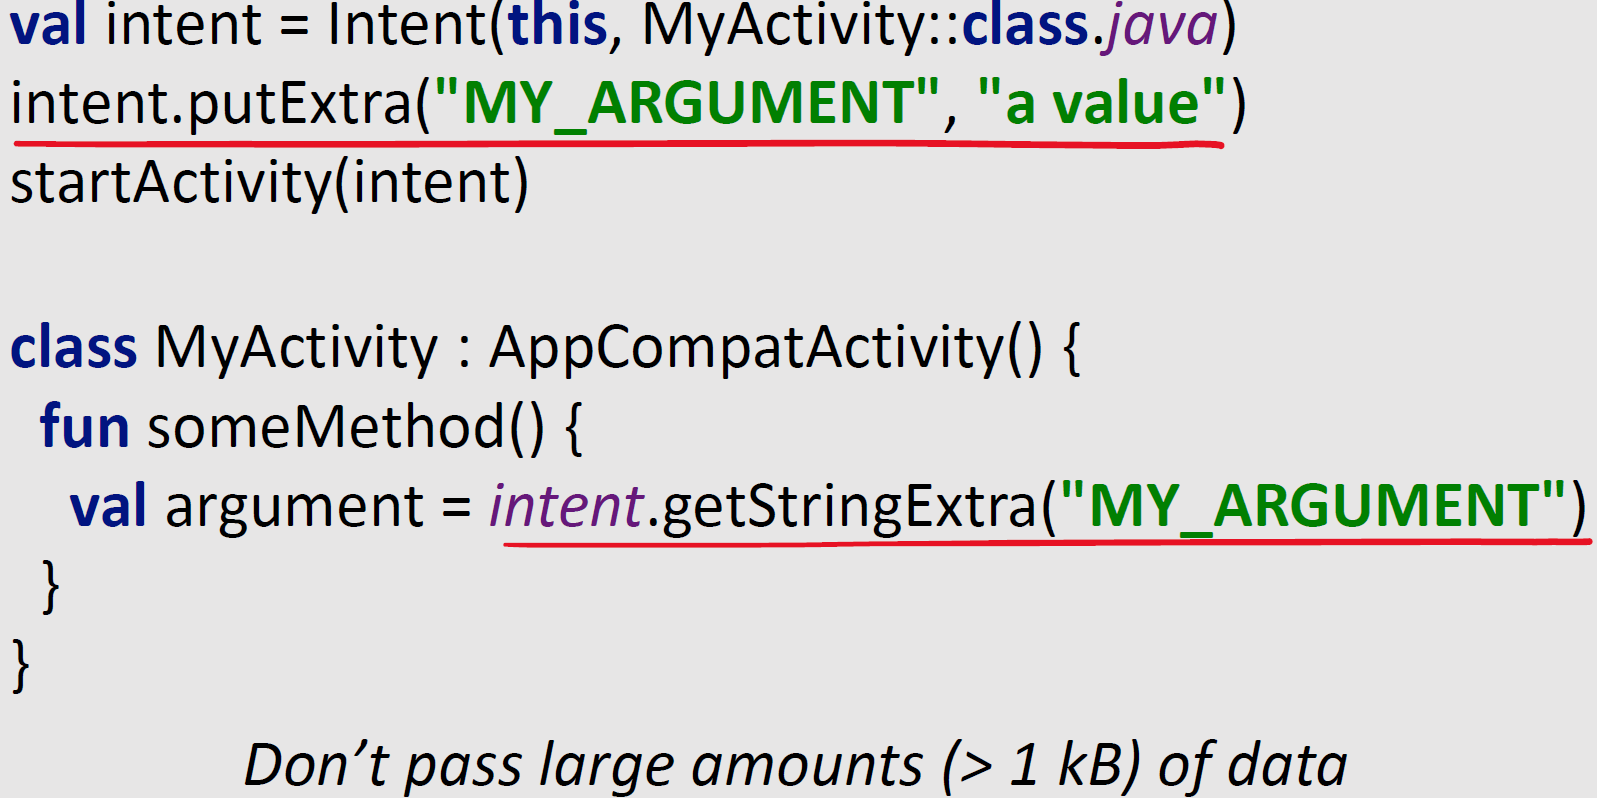
\includegraphics[width=300px]{img/PassingArguments.png}
        \captionof{figure}{Code Snippet passing arguments}
        \label{fig:Code Snippet passing arguments}
\end{Figure}

\subsection{Real-Life Example}
\begin{Figure}
   \centering
    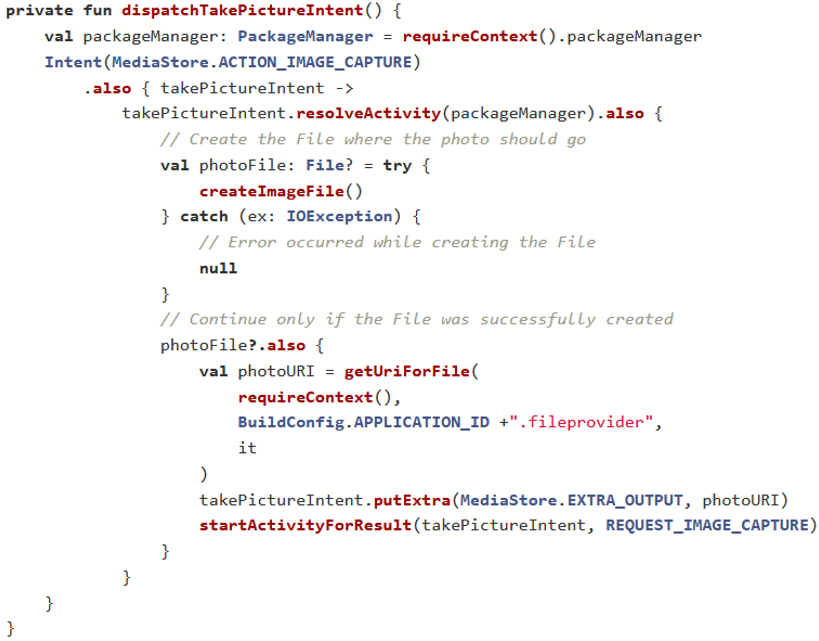
\includegraphics[width=300px]{img/realLifeIntent.png}
        \captionof{figure}{Code Snippet Photo intent from neophyta project}
        \label{fig:Code Snippet Photo intent from neophyta project}
\end{Figure}

\section{Application Object aka Single Thread}
\begin{Figure}
   \centering
    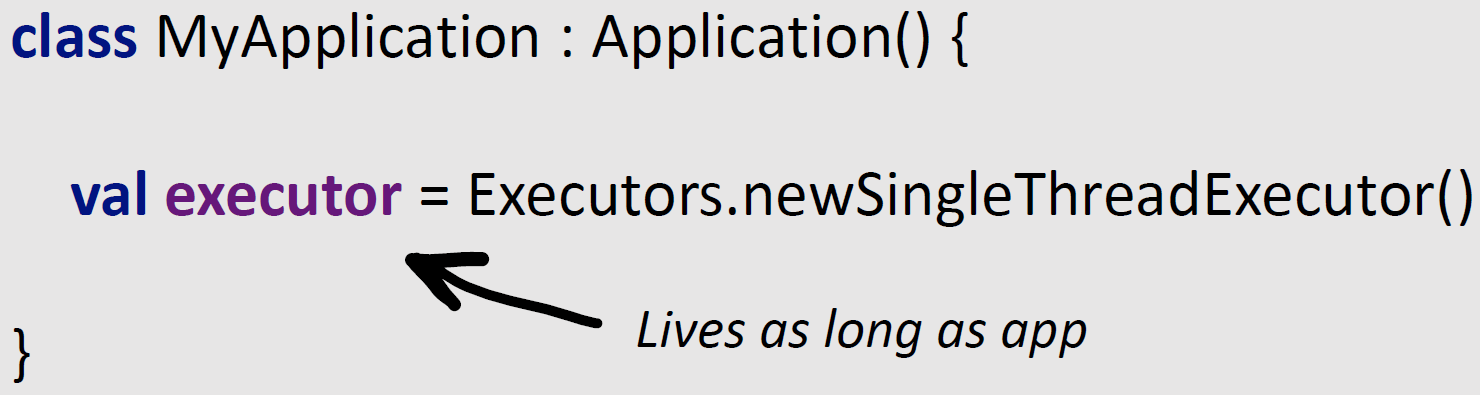
\includegraphics[width=300px]{img/singleThread.png}
        \captionof{figure}{Code Snippet Creating single Thread which lives as long as app}
        \label{fig:Code Snippet Creating single Thread which lives as long as app}
\end{Figure}

\section{Handling Events}
\begin{Figure}
   \centering
    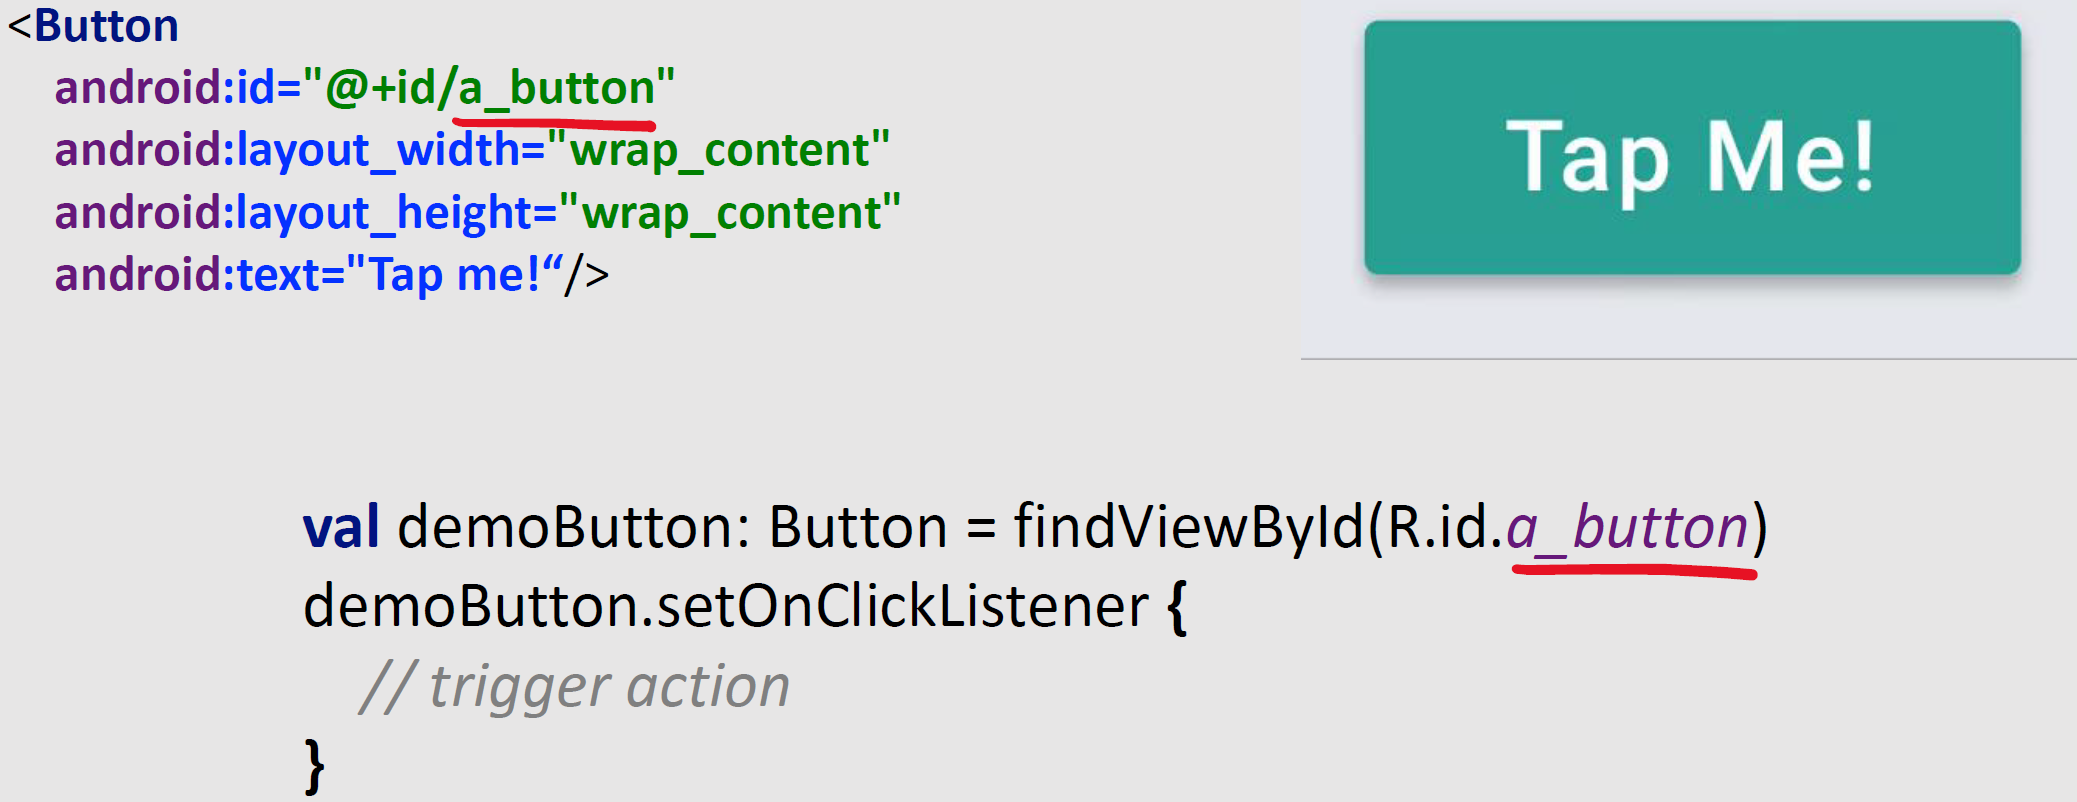
\includegraphics[width=300px]{img/HandlingEvents.png}
        \captionof{figure}{Code Snippet handling events}
        \label{fig:Code Snippet handling events}
\end{Figure}

\begin{Figure}
   \centering
    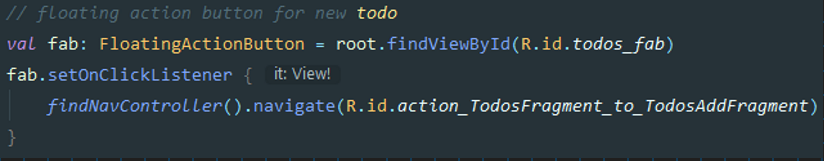
\includegraphics[width=300px]{img/onClickListener.png}
        \captionof{figure}{Code Snippet handling events with trigger action}
        \label{fig:Code Snippet handling events with trigger action}
\end{Figure}

\section{Accessing Ressources}
\begin{Figure}
   \centering
    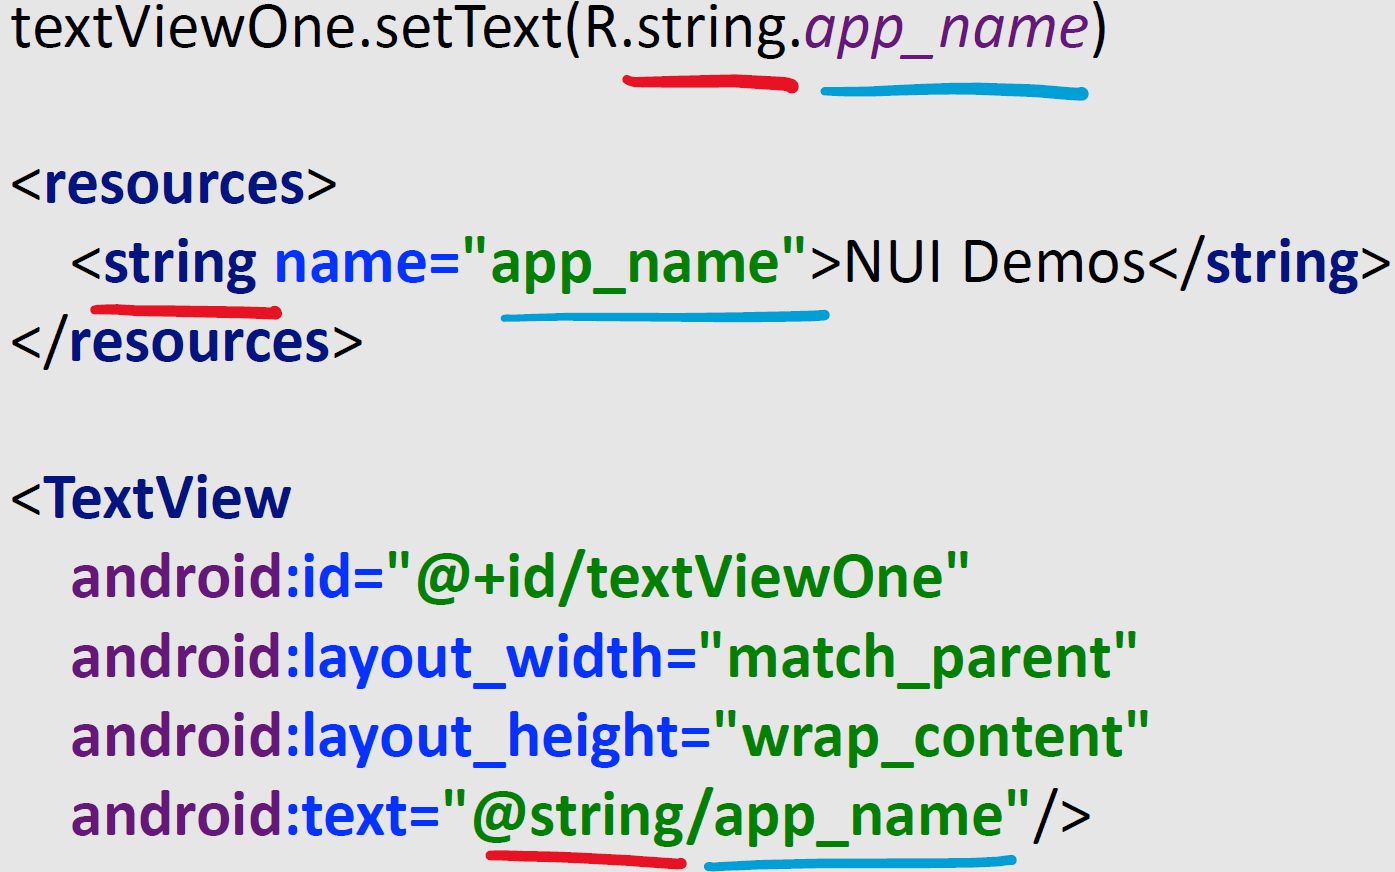
\includegraphics[width=300px]{img/AccessingRessources.png}
        \captionof{figure}{Code Snippet how to access to ressources}
        \label{fig:Code Snippet how to access to ressources}
\end{Figure}

\section{System Ressources}
\begin{Figure}
   \centering
    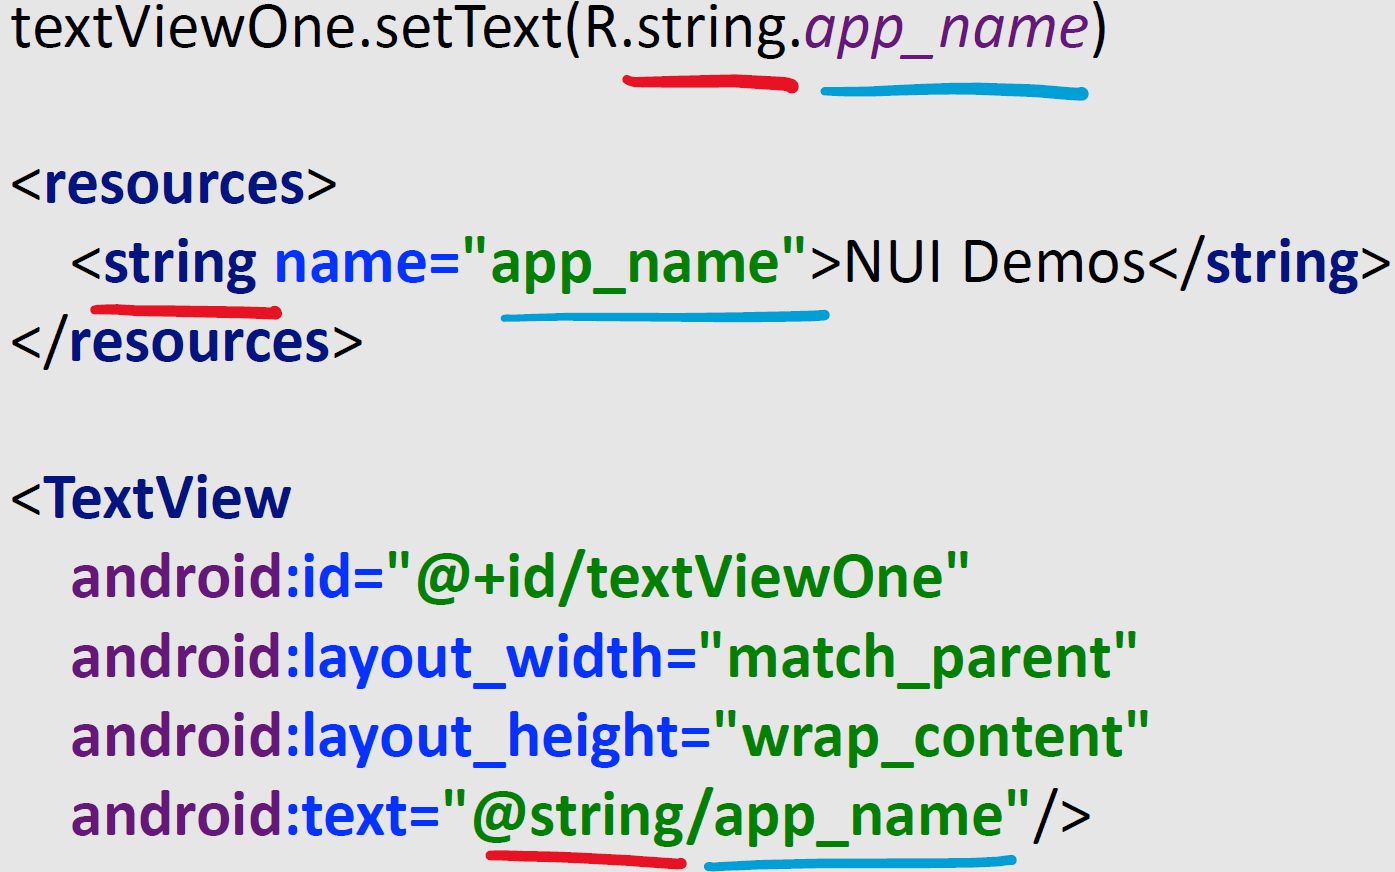
\includegraphics[width=300px]{img/AccessingRessources.png}
        \captionof{figure}{Code Snippet how to access to ressources}
        \label{fig:Code Snippet how to access to ressources}
\end{Figure}

\section{UI Thread}
\begin{Figure}
   \centering
    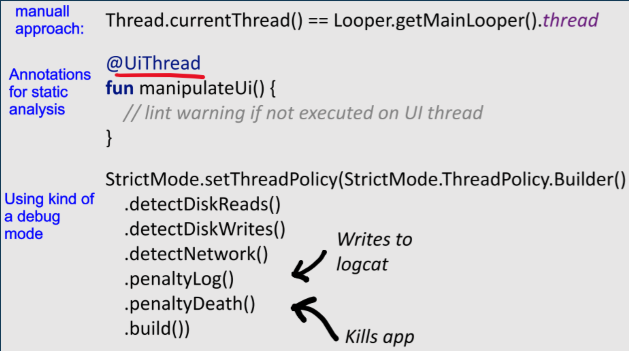
\includegraphics[width=300px]{img/detectingThreadingIssues.png}
        \captionof{figure}{Code Snippet different var for handling UI Threads}
        \label{fig:Code Snippet different var for handling UI Threads}
\end{Figure}

\section{Callback to UI Thread}
\begin{Figure}
   \centering
    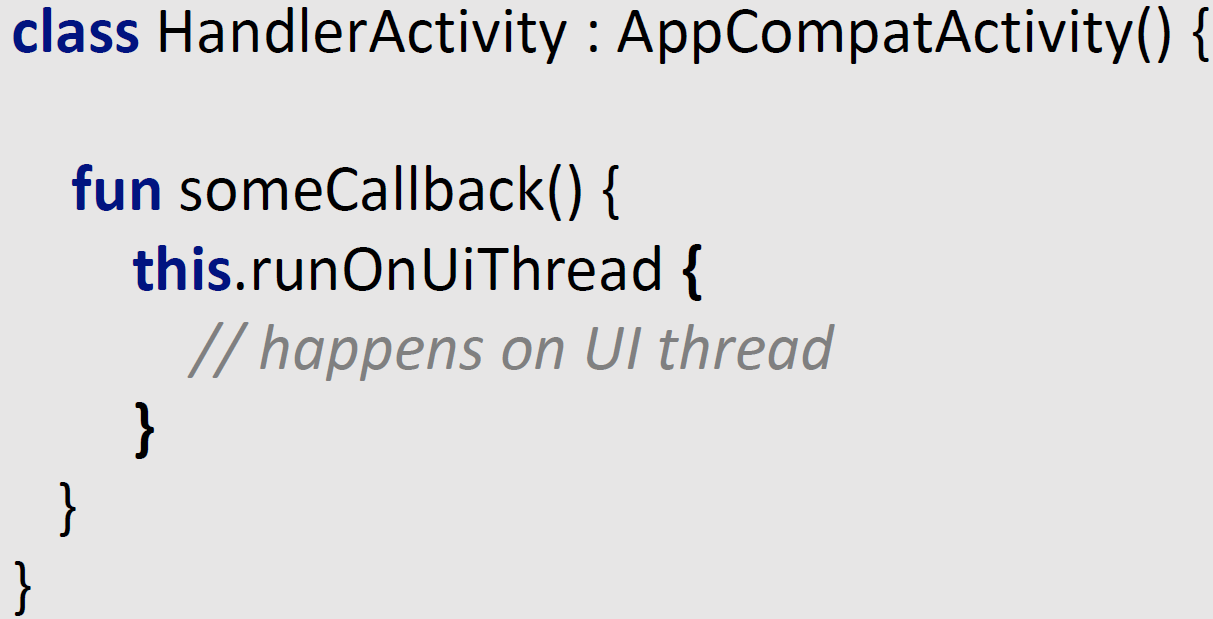
\includegraphics[width=300px]{img/CallbackUIThreadI.png}
        \captionof{figure}{Code Snippet how to implement a Callback to UI Thread V1}
        \label{fig:Code Snippet how to implement a Callback to UI Thread V1}
\end{Figure}
\begin{Figure}
   \centering
    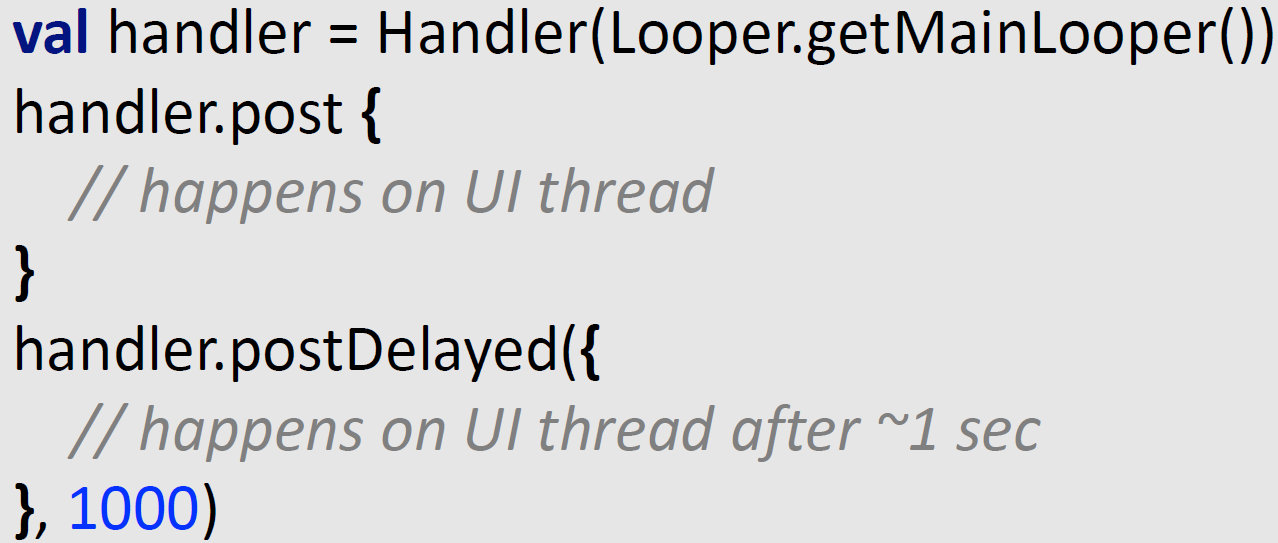
\includegraphics[width=300px]{img/CallbackUIThreadII.png}
        \captionof{figure}{Code Snippet how to implement a Callback to UI Thread V2}
        \label{fig:Code Snippet how to implement a Callback to UI Thread V2}
\end{Figure}

\section{Adapter-Class - Fast-List}

\subsection{Adapter Class extends Viewholder}
\begin{Figure}
   \centering
    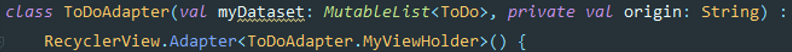
\includegraphics[width=300px]{img/adapterClass.png}
        \captionof{figure}{Code Snippet implement adapter class}
        \label{fig:Code Snippet implement adapter class}
\end{Figure}

\subsection{viewholder}
\begin{Figure}
   \centering
    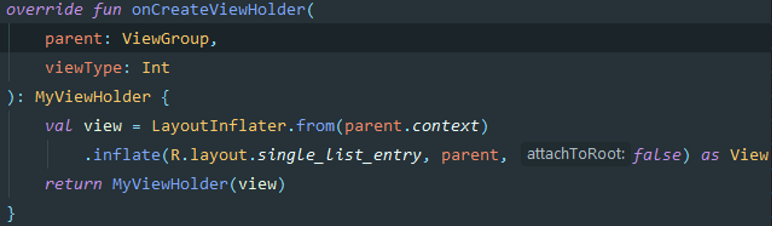
\includegraphics[width=300px]{img/viewholder.png}
        \captionof{figure}{Code Snippet creating a viewholder}
        \label{fig:Code Snippet creating a viewholder}
\end{Figure}

\subsection{onBindViewHolder}
\begin{Figure}
   \centering
    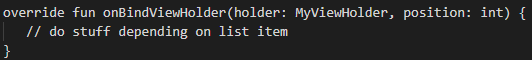
\includegraphics[width=300px]{img/onBindViewHolder.png}
        \captionof{figure}{Code Snippet onBindViewHolder is specific to app, problem, list entry}
        \label{fig:Code Snippet onBindViewHolder is specific to app, problem, list entry}
\end{Figure}

\subsection{Java}
\textbf{onCreateViewHolder(ViewGroup, int)}: This method is called right when the adapter is created and is used to initialize your ViewHolder(s).\\

\textbf{getItemViewType(int)}: This method returns an `Integer` which represents the view type. Since the Android system stores a static reference to each layout as an `Integer` in the “R” (resources) class, we can simply return the layout resource id to be used in the `onCreateViewHolder()` method.\\

\textbf{getItemCount()}: This method returns the size of the collection that contains the items we want to display\\

\textbf{onBindViewHolder(RecyclerView.ViewHolder, int)}: This method is called for each ViewHolder to bind it to the adapter. This is where we will pass our data to our ViewHolder.\\

\begin{Figure}
   \centering
    \includegraphics[width=300px]{img/adapterinJava.png}
        \captionof{figure}{Code Snippet adapter in Java}
        \label{fig:Code Snippet adapter in Java}
\end{Figure}

\section{PresentationModel}
\begin{Figure}
   \centering
    \includegraphics[width=300px]{img/presentationModel.png}
        \captionof{figure}{Code Snippet presentation Model}
        \label{fig:Code Snippet presentation Model}
\end{Figure}


\end{document}
